% Options for packages loaded elsewhere
\PassOptionsToPackage{unicode}{hyperref}
\PassOptionsToPackage{hyphens}{url}
\PassOptionsToPackage{dvipsnames,svgnames,x11names}{xcolor}
\documentclass[
  11pt,
  a4paper,
  oneside]{report}
\usepackage{xcolor}
\usepackage[margin=2.6cm]{geometry}
\usepackage{amsmath,amssymb}
\setcounter{secnumdepth}{5}
\usepackage{iftex}
\ifPDFTeX
  \usepackage[T1]{fontenc}
  \usepackage[utf8]{inputenc}
  \usepackage{textcomp} % provide euro and other symbols
\else % if luatex or xetex
  \usepackage{unicode-math} % this also loads fontspec
  \defaultfontfeatures{Scale=MatchLowercase}
  \defaultfontfeatures[\rmfamily]{Ligatures=TeX,Scale=1}
\fi
\usepackage{lmodern}
% Portable Times-family body font; works under pdflatex (Overleaf
% default) with no external fonts required.
\usepackage{mathptmx}
% Use upquote if available, for straight quotes in verbatim environments
\IfFileExists{upquote.sty}{\usepackage{upquote}}{}
\IfFileExists{microtype.sty}{% use microtype if available
  \usepackage[]{microtype}
  \UseMicrotypeSet[protrusion]{basicmath} % disable protrusion for tt fonts
}{}
\makeatletter
\@ifundefined{KOMAClassName}{% if non-KOMA class
  \IfFileExists{parskip.sty}{%
    \usepackage{parskip}
  }{% else
    \setlength{\parindent}{0pt}
    \setlength{\parskip}{6pt plus 2pt minus 1pt}}
}{% if KOMA class
  \KOMAoptions{parskip=half}}
\makeatother
\setlength{\emergencystretch}{3em} % prevent overfull lines
\providecommand{\tightlist}{%
  \setlength{\itemsep}{0pt}\setlength{\parskip}{0pt}}
\usepackage[]{natbib}
\bibliographystyle{plainnat}
\PassOptionsToPackage{round,authoryear}{natbib}
\usepackage{microtype}
\usepackage{booktabs}
\usepackage{longtable}
\usepackage{array}
\usepackage{amsmath}
\usepackage{amsthm}
\usepackage{amssymb}
\usepackage{graphicx}
\graphicspath{{./}{../}{../../}}
\newtheorem{lemma}{Lemma}
\newtheorem{theorem}{Theorem}
\newtheorem{proposition}{Proposition}
\usepackage{caption}
\captionsetup{font=small,labelfont=bf}
\usepackage{titlesec}
\titleformat{\chapter}[display]{\normalfont\huge\bfseries}{\chaptertitlename\ \thechapter}{20pt}{\Huge}
\titlespacing*{\chapter}{0pt}{-30pt}{20pt}
\usepackage{fancyhdr}
\pagestyle{fancy}
\fancyhf{}
\fancyhead[L]{\nouppercase{\leftmark}}
\fancyhead[R]{\thepage}
\renewcommand{\headrulewidth}{0.4pt}
\usepackage{setspace}
\onehalfspacing
\usepackage[hang,flushmargin]{footmisc}
\setcounter{secnumdepth}{3}
\setcounter{tocdepth}{2}
\usepackage{xurl}
\urlstyle{tt}
\renewcommand{\UrlFont}{\scriptsize\ttfamily}
\usepackage{seqsplit}
\hyphenpenalty=50
\exhyphenpenalty=50
\tolerance=3000
\emergencystretch=3em
\usepackage{etoolbox}
\renewcommand{\maketitle}{}
\bibliographystyle{plainnat}
\AtBeginDocument{\bibpunct{(}{)}{;}{a}{,}{,}}
\usepackage{bookmark}
\IfFileExists{xurl.sty}{\usepackage{xurl}}{} % add URL line breaks if available
\urlstyle{same}
\hypersetup{
  pdftitle={A Self-Financed Wagering Mechanism with Online Skill Learning},
  pdfauthor={Anastasia Cattaneo},
  colorlinks=true,
  linkcolor={Maroon},
  filecolor={Maroon},
  citecolor={Blue},
  urlcolor={Blue},
  pdfcreator={LaTeX via pandoc}}

\title{A Self-Financed Wagering Mechanism with Online Skill Learning}
\usepackage{etoolbox}
\makeatletter
\providecommand{\subtitle}[1]{% add subtitle to \maketitle
  \apptocmd{\@title}{\par {\large #1 \par}}{}{}
}
\makeatother
\subtitle{Forecast Aggregation under Budget Balance, Truthfulness and
Sybil-Proofness}
\author{Anastasia Cattaneo}
\date{\today}

\begin{document}
\maketitle

\begin{titlepage}
\begin{center}
\vspace*{4em}
{\Huge\bfseries A Self-Financed Wagering Mechanism\\[0.5em] with Online Skill Learning\par}
\vspace{1.5em}
{\Large Forecast aggregation under budget balance, truthfulness, and sybil-proofness\par}
\vspace{4em}
{\Large Anastasia Cattaneo\par}
\vspace{1em}
{\large Imperial College London\par}
\vspace{4em}
{\large MSc Thesis \\ \today\par}
\vfill
\end{center}
\end{titlepage}

\pagenumbering{roman}

\chapter*{Abstract}
\addcontentsline{toc}{chapter}{Abstract}

Prediction markets for probabilistic forecasts face a design tension:
existing self-financed wagering mechanisms
\citep{lambert2008selffinanced,
raja2024wagering} satisfy strong axioms (budget balance, truthfulness,
sybil-proofness) but treat each round in isolation, while
online-learning aggregators \citep{vitali2025intermittent} adapt to
participant reliability but relax self-financing. This thesis resolves
the tension by placing an online skill layer on top of the
weighted-score wagering mechanism. A bounded scalar skill \(\sigma_i\),
an exponentially weighted moving average of each participant's past
pinball loss, modulates the deposit before every round into an effective
wager that governs both aggregation weight and settlement exposure.
Because the modulation is pre-round and measurable under the history up
to \(t-1\), Lambert's per-round proofs carry over verbatim. The
mechanism is verified to preserve budget balance to machine precision
and the narrow Lambert sybil invariance to floating-point noise. On a
controlled known-noise panel the Spearman correlation between learned
\(\sigma\) and ground-truth CRPS equals one. On 17,344 hours of Elia
offshore-wind power the mechanism reduces CRPS by \(7.1\%\) against
uniform averaging (Diebold--Mariano \(t = 40.77\), \(p \approx 0\)); on
10,000 rounds of electricity-imbalance prices the mechanism is
indistinguishable from uniform (\(t = 0.008\), \(p = 0.994\)), a regime
consistent with the forecast-combination puzzle
\citep{timmermann2006forecast}. A rolling isotonic recalibration
\citep{kuleshov2018accurate} closes \(41\%\) of the tail-calibration gap
at a \(1.6\%\) CRPS cost. Against a theory-grounded adversary catalogue,
the mechanism inherits the \citet{chen2014arbitrage} arbitrage
vulnerability but preserves sybil invariance under identical clone
reports; diversified clones and coalitions remain profitable and are
documented as limitations.

\vspace{1em}

\noindent\textbf{Keywords.} prediction markets; self-financed wagering
mechanism; online learning; forecast aggregation; continuous ranked
probability score; budget balance; sybil-proofness; isotonic
recalibration; offshore wind power.

\chapter*{Acknowledgements}
\addcontentsline{toc}{chapter}{Acknowledgements}

I thank my supervisor for supporting the direction of this work and for
pointing me to the \citet{vitali2025intermittent} manuscript early in
the project. I thank Elia for publishing the offshore-wind and
electricity-imbalance data used in the empirical chapters. Errors and
omissions are my own.

\cleardoublepage
\tableofcontents
\cleardoublepage

\pagenumbering{arabic}

\chapter{Introduction}\label{ch:intro}

\section{Motivation}\label{motivation}

Decisions under uncertainty in modern energy systems depend on accurate
short-horizon forecasts. Balancing a power system, scheduling reserves,
clearing intraday markets, and settling imbalance positions all rest on
expectations of generation or load that are updated continuously as new
information arrives. The relevant information is rarely concentrated in
a single actor. Independent operators, aggregators, and analysts each
see part of the signal: one may operate a superior
numerical-weather-prediction chain, another a locally tuned
machine-learning model, a third hold private telemetry from installed
assets. Raw data are typically commercially sensitive or expensive to
share, yet a derived forecast can be communicated without exposing the
underlying inputs.

This observation motivates the study of \emph{prediction markets} for
forecasts. A market operator posts a prediction task; participants
submit a probabilistic forecast together with a wager; the operator
aggregates the reports into a single collective forecast and, once the
outcome is observed, redistributes the wager pool according to a scoring
rule. When the mechanism is \emph{self-financed}, in the sense that the
sum of post-event payouts equals the sum of pre-event wagers, no
external subsidy is required and the market can run indefinitely on its
own accounting. \citet{lambert2008selffinanced} formalised this class as
the \emph{weighted-score wagering mechanism} and proved that, under five
axioms, budget balance, anonymity, truthfulness, normality, and
sybil-proofness, it is the unique mechanism satisfying all five
simultaneously.

Two limitations of the Lambert formulation are salient for practical
deployment. First, each round is treated in isolation: the mechanism
makes no use of the fact that, in most applications, the same
participants return round after round and differ systematically in
reliability. Second, the formulation assumes full participation: a
participant who misses a round simply does not play, with no bookkeeping
consequence for future rounds. Both assumptions are violated in energy
prediction markets, where skill is persistent and participation is
intermittent. \citet{vitali2025intermittent} addressed the second
limitation directly with an online-gradient-descent aggregator that
tracks historical performance and tolerates missing submissions, but at
the cost of relaxing self-financing: a separate payoff-allocation step
is introduced, and Lambert's axiomatic guarantees no longer apply.

This thesis bridges the two strands. We introduce an online
skill-learning layer that sits on top of the weighted-score wagering
mechanism without disturbing its settlement algebra. Each participant's
deposit is modulated, before every round, by a bounded scalar
\emph{skill estimate} computed as an exponentially weighted moving
average of that participant's past probabilistic losses. The resulting
\emph{effective wager} \[
  m_i = b_i \cdot \big(\lambda + (1-\lambda)\, \sigma_i^{\eta}\big)
\] is the single object that governs both aggregation weight and
financial exposure. Because the modulation is a scalar multiplier
applied pre-round and derived exclusively from information strictly
earlier than the current report, the Lambert truthfulness proof applies
verbatim with the modulated wager \(m_i\) in place of the original
deposit \(b_i\).

\section{Research question}\label{research-question}

The thesis is organised around a single question in three parts: when
predictive information is distributed across many participants, how
should their forecasts be combined, and how should the market decide
whose forecast deserves more influence, while preserving the budget
balance, truthfulness, and sybil-proofness that make the mechanism
credible?

Three sub-questions follow:

\begin{enumerate}
  \item Can a market learn participant reliability from data alone,
    online, without an external subsidy, and can that learning be
    proved convergent on data with known latent skill?
  \item Does using the learned reliability to weight the aggregate
    forecast improve accuracy on real energy data, and if so under
    what conditions?
  \item Can the extension be carried out while preserving Lambert's
    axiomatic guarantees and without opening new strategic attack
    surfaces beyond those already present in any weighted-score
    wagering mechanism?
\end{enumerate}

The answer developed across the remainder of the thesis is a conditional
affirmative on all three sub-questions. The conditions are stated
explicitly and are tied to measurable properties of the forecaster panel
and the underlying data-generating process.

\section{Contributions}\label{contributions}

The thesis makes five primary contributions.

First, a self-financed wagering mechanism that couples weighted-score
settlement with an online, absolute, pre-round skill signal. The
effective wager
\(m_i = b_i \cdot (\lambda + (1-\lambda)\,\sigma_i^{\eta})\) controls
both aggregation weight and settlement exposure. Lambert's truthfulness
proof \citep{lambert2008selffinanced} is preserved under the
substitution \(m_i \leftarrow b_i\), and budget balance holds by
construction.

Second, empirical verification of correctness. The mechanism satisfies
all thirteen active Lambert combinatorial payoff invariants on the
reference implementation, supported by eighty golden-value regression
snapshots across sixteen payoff-module functions. Budget balance holds
to machine precision (maximum absolute gap \(2.84 \times 10^{-14}\)
across 1000 synthetic rounds); the narrow Lambert sybil invariance holds
with mean profit ratio \(1.000000\) and maximum absolute deviation
\(2.07 \times 10^{-17}\).

Third, skill recovery on controlled data. On a known-noise synthetic
panel (six forecasters, \(T = 20{,}000\) rounds, twenty seeds), the
Spearman rank correlation between the true noise scale and the learned
skill estimate \(\sigma\) equals one in both point-forecast and
quantile-forecast modes. The learned \(\sigma\) values are monotone in
the true noise scale across the range \([0.15, 1.00]\).

Fourth, identification of deposit design as the dominant empirical
lever. A four-way deposit-policy ablation shows that bankroll-confidence
deposits, computed from observable quantities alone, reduce CRPS by
\(10.4\%\) against fixed-unit deposits, capturing approximately one
quarter of the improvement attained by an oracle-precision deposit.
Holding the deposit policy fixed, the choice of weighting rule moves
CRPS by at most a few percent, while the deposit policy moves it by tens
of percent.

Fifth, real-data validation on two Elia series. On the full
17\{,\}344-hour offshore-wind series under strictly-causal expanding
normalisation, the mechanism reduces CRPS by \(7.1\%\) relative to
uniform averaging (Diebold--Mariano \(t = 40.77\), \(p \approx 0\)). On
electricity-imbalance prices (\(T = 10{,}000\)), the mechanism is
statistically indistinguishable from uniform (\(t = 0.008\),
\(p = 0.994\)) because the seven forecasters produce near-identical
CRPS; this null result is reported rather than suppressed. Against
Elia's published real-time operational forecast, which attains
74.0\textasciitilde MW in CRPS-megawatt-equivalent units, the mechanism
reaches 83.7\textasciitilde MW and the best single forecaster, an online
gradient-boosted tree model trained on the observed series with no
weather inputs, reaches 69.5\textasciitilde MW.

In addition, the quantile-averaged aggregate is miscalibrated in the
manner analogous to \citet{ranjan2010combining}'s linear-pool
impossibility, with a mean tail deviation of \(0.019\) on the audit
slice, exhibiting under-coverage in the lower tail and over-coverage in
the mid-upper range. A rolling isotonic recalibration following
\citet{kuleshov2018accurate} closes \(41\%\) of the tail deviation at a
CRPS cost of \(1.6\%\) and a sharpness cost of \(12\%\), without
modifying the skill, wager, aggregation, or settlement layers. Eight
theory-grounded adversaries, arbitrage \citep{chen2014arbitrage},
Chun--Shachter coalitions \citep{chun2011cooperating}, informed
collusion, a lagged insider \citep{johnstone2007economic}, wash trading,
strategic reporting, detector-aware evasion, and sybil arbitrage, are
evaluated across ten to twenty paired seeds with \(95\%\) confidence
intervals. The narrow Lambert sybil invariance holds to floating-point
noise; diversified-report sybils break the invariance by approximately
\(6.5\%\); arbitrage profit scales monotonically with \(\lambda\), from
\(+11.68\) at \(\lambda = 0\) to \(+24.22\) at \(\lambda = 1\) over 1000
rounds.

\section{Structure of the thesis}\label{structure-of-the-thesis}

Chapter\textasciitilde{}\ref{ch:related} reviews the three strands on
which the thesis builds: self-financed wagering mechanisms, online
forecast combination, and probabilistic forecast evaluation.
Chapter\textasciitilde{}\ref{ch:mechanism} specifies the mechanism:
round structure, skill gate, and settlement algebra. It argues why
making the effective wager the single object that governs both influence
and exposure preserves Lambert's axioms.
Chapter\textasciitilde{}\ref{ch:methodology} describes the datasets, the
forecaster panel, and the experimental protocol.
Chapter\textasciitilde{}\ref{ch:synthetic} reports synthetic validation:
mechanism correctness, skill recovery, deposit-policy ablation,
weight-rule comparison, and a five-step bankroll-pipeline ablation.
Chapter\textasciitilde{}\ref{ch:real} reports real-data results on Elia
offshore wind and electricity-imbalance prices, together with an
external validation against Elia's own operational forecast.
Chapter\textasciitilde{}\ref{ch:recalibration} develops a rolling
isotonic recalibration layer as a post-hoc remedy for the
\citet{ranjan2010combining} linear-pool miscalibration.
Chapter\textasciitilde{}\ref{ch:robustness} evaluates the mechanism
against the theory-grounded adversary catalogue.
Chapter\textasciitilde{}\ref{ch:discussion} discusses limitations,
scope, and threats to validity, and
Chapter\textasciitilde{}\ref{ch:conclusion} concludes.

\section{Scope}\label{scope}

For clarity, the following are out of scope. We do not propose a new
scoring rule: CRPS and the pinball loss, both strictly proper
\citep{gneiting2007strictly}, are used unchanged. We do not replace
Lambert's settlement algebra; the skill layer is a pre-round
multiplicative modulator on the wager, with no post-round
re-normalisation, no side payments, and no change to the redistribution
law. We do not overturn the \citet{ranjan2010combining} impossibility:
the aggregate is uncalibrated for the reason their theorem predicts, and
the recalibration layer closes part of the gap post-hoc without claiming
to remove the underlying obstruction. We do not claim sybil-proofness
under arbitrary report diversity; the Lambert axiom applies to identical
reports with conserved total wager, and we verify the narrow invariance
numerically while measuring the empirical leakage under small
report-diversification attacks. Finally, we do not characterise
coalition equilibria or best-response dynamics: the robustness chapter
tests eight named adversary strategies with published theoretical bases
and reports attacker profit with confidence intervals, without computing
Nash or correlated equilibria.

\chapter{Related work}\label{ch:related}

This chapter reviews the three research strands on which the thesis
builds: self-financed wagering mechanisms, online learning for forecast
combination, and probabilistic forecast evaluation and calibration. The
structure follows the logical dependencies of the mechanism developed in
Chapter 3 rather than a strict chronology.

\section{Self-financed wagering
mechanisms}\label{self-financed-wagering-mechanisms}

The foundational result is due to \citet{lambert2008selffinanced}, who
defined a wagering mechanism as a triple of report vector, outcome
space, and payoff function, and identified seven axiomatic properties:
budget balance, anonymity, truthfulness, sybil-proofness, normality,
individual rationality, and monotonicity. They showed that the
single-parameter weighted-score mechanism with payoff \[
  \Pi_i(r, m, \omega) = m_i \left( 1 + s(r_i, \omega)
    - \frac{\sum_j s(r_j, \omega)\, m_j}{\sum_j m_j} \right)
\] satisfies all seven, and that it is the unique mechanism satisfying
the first five. Sybil-proofness is proved for the case in which clones
report identically and the total wager is conserved, a scope
qualification that recurs throughout the later literature. Our mechanism
preserves this payoff form exactly, substituting the effective wager
\(m_i\) for the raw deposit, so that the Lambert truthfulness and sybil
proofs apply unchanged on a per-round basis.

\citet{raja2024wagering} extended the framework from binary or discrete
outcomes to continuous outcomes and probabilistic quantile forecasts, in
the setting of an energy-sector prediction market with an explicit
buyer. They showed that the payoff mechanism retains budget balance,
truthfulness, sybil-proofness, and individual rationality in the
quantile setting. Each market instance remains history-free: no
inter-round state is accumulated. The online skill layer developed in
Chapter 3 is precisely the component that accumulates such state across
rounds while keeping the per-round payoff algebra intact.

The arbitrage properties of weighted-score mechanisms were characterised
by \citet{chen2014arbitrage}. They showed that, for any differentiable
strictly proper scoring rule, participant \(i\) can choose a report in
an \emph{arbitrage interval} that yields a non-negative payoff under
every outcome, strictly positive whenever other participants disagree
(their Theorem 3.3). The arbitrage-seeking adversary studied in Chapter
8 implements the mean-absolute-error analogue of this arbitrage point,
namely the wager-weighted median of other reports, and participates only
when the expected profit under a uniform outcome is strictly positive.
Empirically this extracts \(+12\) to \(+24\) cumulative profit per 1000
rounds across our \(\lambda\) grid, confirming the theorem.
\citet{chen2014arbitrage} also constructed a family of no-arbitrage
wagering mechanisms that preserve anonymity, individual rationality,
incentive compatibility, weak budget balance, and sybil-proofness for
the \(f\)-NAWM subclass. Moving to that family is out of scope here; the
contribution of the present thesis is the composition of budget balance
with an online skill layer and a post-hoc calibration layer, not the
removal of arbitrage.

\citet{chun2011cooperating} studied coalitions in strictly-proper
elicitation. They showed that a coalition \(C\) of participants with
immutable beliefs who all report the common value
\[p_C = \sum_{i \in C} \frac{w_i}{W_C}\, p_i, \qquad
  W_C = \sum_{i \in C} w_i,\] earns a strictly higher total payoff than
reporting truthfully, whenever coalition members disagree. This formula
provides the specification for the coordinated-group adversary evaluated
in Chapter 8; combined with a privileged lagged signal under an AR(1)
outcome process, the attack attains cumulative profit of \(+33.84\) per
1000 rounds.

Two further works are relevant as framing. \citet{dimitrov2008nonmyopic}
observed that rational non-myopic forecasters in repeated prediction
markets may report off-belief values to mislead competitors before
correcting, and that a discount factor can blunt the incentive.
\citet{johnstone2007economic} provided the informational framing adopted
for our insider-advantage experiment: in a repeated wagering setting, a
forecaster with superior information accumulates wealth at a rate
determined by the Kullback--Leibler divergence between her belief and
the market's belief. The insider adversary in Chapter 8 replaces the
hard leak of the outcome with a low-variance lagged signal, aligning the
attack with this informational model.

Reputation attacks on participant-identity systems form a distinct
literature. The relevant precedent is \citet{feldman2004freeriding}, who
catalogued the \emph{whitewashing} attack, in which a participant
abandons a degraded reputation and re-enters as a newcomer, and showed
that a penalty on every newcomer partly offsets the incentive. The
reputation-reset adversary in Chapter 8 tests this attack against the
skill layer; the staleness decay \(\kappa\) together with the non-unit
prior \(\sigma_{\mathrm{init}}\) realises the newcomer-penalty
recommendation.

Finally, \citet{witkowski2018forecasting} distinguish self-financed
wagering from incentive-compatible \emph{forecasting competitions}. In a
winner-take-all tournament, forecasters have an incentive to report
extreme beliefs so as to maximise the probability of winning, and
truthful reporting requires a different mechanism design. The present
mechanism is a self-financed market, not a tournament; budget balance,
not a fixed prize pool, underwrites per-round truthfulness.

\section{Online learning for forecast
combination}\label{online-learning-for-forecast-combination}

The closest direct antecedent is \citet{vitali2025intermittent}, who
proposed a prediction market that tracks historical performance, adapts
to time-varying conditions, and allows agents to join and leave. They
use robust regression with online gradient descent on the simplex to
learn relative combination weights, and introduce an in-sample plus
out-of-sample payoff allocation. The two approaches differ in four
respects. First, the weights in the present mechanism are absolute
rather than relative: we learn a scalar skill \(\sigma_i\) per
participant, rather than a simplex-constrained weight vector. Second,
the present mechanism is self-financed by construction, inheriting the
Lambert payoff formula, whereas \citet{vitali2025intermittent} relax
self-financing to enable the online-gradient-descent update. Third, a
single object, the effective wager \(m_i\)---governs both aggregation
weight and financial exposure in our design, whereas theirs separates
the two. Fourth, intermittency is handled through a staleness decay
toward a neutral prior, not through robust regression.
Table\textasciitilde{}\ref{tab:vitali-diff} summarises these
differences.

\begin{table}[h]
\centering
\small
\begin{tabular}{lll}
\toprule
& Vitali \& Pinson (2025) & This thesis \\
\midrule
Weights & Relative (simplex), OGD & Absolute (EWMA of loss) \\
Self-financed & No (separate allocation) & Yes (Lambert/Raja inherited) \\
Single object for influence and exposure & No & Yes (effective wager $m_i$) \\
Intermittency & Robust regression & Staleness decay toward prior \\
\bottomrule
\end{tabular}
\caption{Positioning relative to \citet{vitali2025intermittent}.}
\label{tab:vitali-diff}
\end{table}

Their online-gradient-descent variant is retained as a published
reference aggregator throughout the empirical chapters, where it appears
as a shifted-median fan baseline (Chapter 6). The ratio of our mechanism
to this baseline is \(0.985\) on the 3000-point audit slice, a \(1.5\%\)
CRPS advantage for the self-financed design on that slice. On the full
17\{,\}344-hour expanding-mode wind run, the per-quantile OGD baseline
of \citet{vitali2025intermittent} improves on our mechanism by
approximately fourteen percentage points of CRPS; this gap quantifies the
CRPS cost of preserving the Lambert budget-balance guarantee rather than
relaxing to a per-quantile simplex aggregator.

The theoretical grounding of online aggregation is the
regret-minimisation framework of \citet{cesabianchi2006prediction}, in
which the cumulative loss of the aggregator is compared with the
cumulative loss of the best expert in hindsight. \citet{chen2010new}
made the equivalence between market scoring rules and online no-regret
algorithms explicit, which motivates our EWMA skill layer as a
bounded-regret estimator on stationary panels. The EWMA update is
consistent under stationarity by the classical stochastic approximation
result of \citet{robbins1951stochastic}; under non-stationarity, the
tracking error is bounded by \(O(\rho \cdot \mathrm{drift})\), with
\(\rho\) the EWMA learning rate \citep{benveniste1990adaptive}. The
bankroll-confidence deposit policy is a deterministic analogue of the
log-optimal growth criterion of \citet{kelly1956new}, in which the
log-optimal rate is replaced by a bounded monotone function of forecast
spread as a proxy for precision.

The forecast-combination literature provides the canonical baselines
against which any adaptive aggregator must be compared.
\citet{bates1969combination} introduced inverse-variance weighting for
point forecasts, and \citet{timmermann2006forecast} documented the
\emph{combination puzzle}: simple equal weights often outperform
theoretically optimal combinations in practice, owing to estimation
error in the weight parameters. The empirical findings of Chapter 6 are
consistent with this literature. On Elia offshore wind, with sufficient
forecaster heterogeneity and a long evaluation window, the adaptive
skill gate improves on uniform averaging by \(7.1\%\) CRPS; on Elia
electricity-imbalance prices, where the seven forecasters produce
near-identical CRPS, the mechanism is statistically indistinguishable
from uniform, which is the regime the combination puzzle predicts.

Recent work on \emph{performative} prediction
\citep{hardt2023performative, treutlein2023performative} considers the
case in which the forecast itself influences the outcome, creating a
fixed-point problem. We do not model performativity directly, but record
that it would amplify the strategic-reporting threat in Chapter 8:
shifting the aggregate report \(\hat r\) could also shift the outcome
\(y\) that scores the attacker. Extending the skill layer to
performative settings is a natural direction for future work.

\section{Probabilistic forecast evaluation and
calibration}\label{probabilistic-forecast-evaluation-and-calibration}

Scoring rules support both the mechanism's truthfulness argument and its
empirical evaluation. \citet{gneiting2007strictly} defined strict
propriety, a forecaster maximises expected score only by reporting the
true distribution, and showed that the continuous ranked probability
score (CRPS) and the pinball loss are strictly proper.
\citet{steinwart2011estimating} gave the formal statement that pinball
loss is strictly consistent for the \(\tau\)-quantile functional under
mild conditions, which is the elicitability result underlying our
per-round truthfulness argument when participants report quantile grids.

The guiding principle for probabilistic forecast evaluation is due to
\citet{gneiting2007probabilistic}: maximise sharpness subject to
calibration. Sharpness is a property of the forecast alone, whereas
calibration is joint with the observations. The key impossibility is due
to \citet{ranjan2010combining}: any non-trivial weighted average of two
or more distinct calibrated probability forecasts is necessarily
uncalibrated and lacks sharpness. This is the theoretical reason the
mechanism's linear-pool aggregate is miscalibrated, and it motivates the
post-hoc recalibration layer developed in Chapter 7.
\citet{gneiting2013combining} proposed the Beta-transformed linear pool
as a parametric alternative to isotonic recalibration that preserves
sharpness better; this extension is not implemented here and is
identified as future work in Chapter 10.

Our recalibration layer implements the isotonic post-processor of
\citet{kuleshov2018accurate} in a rolling-buffer, prequential
configuration \citep{dawid1984prequential}. Their Theorem 1 gives
asymptotic convergence to calibration under an independent, identically
distributed assumption that cannot be invoked directly for wind and
electricity data. The adversarial, online-regret extension in
\citet{deshpande2023calibrated} relaxes the independence assumption at
the cost of finite-horizon rather than asymptotic calibration
guarantees, and motivates the rolling-buffer design as safer than a
fixed held-out fit under potential non-stationarity.

The evaluation methodology is the prequential framework of
\citet{dawid1984prequential}, in which each observation is first used
for testing and then for training. Practical protocols for time-series
forecasting derive from \citet{tashman2000outofsample}, who formalised
rolling-origin evaluation; \citet{gama2013stream}, who adapted
prequential error estimation to streaming settings; and
\citet{cerqueira2020evaluating}, who empirically compared
performance-estimation methods for time series. We use expanding-window
cross-validation with a 24-step embargo for the XGBoost and
multilayer-perceptron forecasters, following \citet{bergmeir2018note},
who showed this to be a safe default when autocorrelation in residuals
cannot be ruled out. Paired forecast comparisons are reported using the
test of \citet{diebold1995comparing} with heteroscedasticity- and
autocorrelation-consistent standard errors.

\section{Gap statement}\label{gap-statement}

Existing work provides either strong axiomatic structure without online
adaptation \citep{lambert2008selffinanced, raja2024wagering} or online
adaptation without self-financing \citep{vitali2025intermittent}. No
published work combines the two on top of a strictly-proper quantile
scoring rule together with an explicit calibration analysis. The present
thesis addresses this gap.

\chapter{Mechanism design}\label{ch:mechanism}

This chapter specifies the mechanism in full. Throughout, subscript
\(i \in \{1, \dots, n\}\) ranges over participants and subscript \(t\)
over rounds. Vectors over participants are written in bold. The notation
follows \citet{lambert2008selffinanced} where compatible and departs
from it only where the online skill layer requires additional structure.

\section{Round structure}\label{round-structure}

Each round consists of five steps. Every step is a pure function of the
mechanism's persistent state and the current round's inputs, with no
forward references to the outcome. The steps are, in order, submission,
the skill gate, aggregation, scoring and settlement, and the state
update.

\begin{figure}[h]
\centering

\includegraphics[width=0.95\textwidth]{figures/mechanism_steps.png}
\caption{Five-step per-round pipeline. Participants submit quantile
forecasts and deposits; the skill gate modulates the deposit into
an effective wager; the effective wagers define aggregation weights;
once the outcome is realised the pinball-based score drives a
Lambert-form settlement; finally, the exponentially weighted loss
updates the skill estimate for round $t+1$.}
\label{fig:mechanism-steps}
\end{figure}

\subsection{Step 1: submission}\label{step-1-submission}

Each participant \(i\) submits a probabilistic forecast as a vector of
quantiles \(q_i(\tau_k)\) for \(k = 1, \dots, K\), together with a
deposit \(b_i\) drawn from her wealth \(W_i\). The quantile grid is
fixed to \(K = 9\) equidistant levels \(\{0.1, 0.2, \dots, 0.9\}\).

The deposit policy determines how much information is encoded in the
stake. Three regimes are studied:

\begin{itemize}
  \item \textbf{Fixed} ($b_i = 1$), which isolates the skill signal
  from any wealth feedback.
  \item \textbf{Bankroll-fraction}
  $b_i = \min\big(W_i,\, b_{\max},\, f \cdot W_i \cdot c_i\big)$,
  where $c_i = \mathrm{clip}\!\big(\exp(-\beta_c \cdot \Delta_i),
  c_{\min}, c_{\max}\big)$ and $\Delta_i = q_i(0.9) - q_i(0.1)$ is the
  $80\%$-interval width of the forecast. Narrower forecasts produce
  larger $c_i$. For the per-round truthfulness argument,
  $c_i$ is always computed from lagged reports. This is a heuristic
  design choice: the deterministic analogue of fractional-Kelly
  betting \citep{kelly1956new}, replacing the log-optimal growth rate
  with a bounded monotone function of forecast spread as a proxy for
  precision. It is not itself induced by a proper scoring rule.
  \item \textbf{Oracle-precision} ($b_i \propto$ true signal
  precision), which is not implementable in practice and serves as
  the theoretical ceiling.
\end{itemize}

\subsection{Step 2: skill gate}\label{step-2-skill-gate}

The deposit is modulated by a bounded, absolute skill estimate
\(\sigma_i \in [\sigma_{\min}, 1]\) to give the effective wager:
\begin{align}
  m_i &= b_i \cdot g(\sigma_i), \\
  g(\sigma) &= \lambda + (1 - \lambda)\, \sigma^{\eta}, \\
  \mathrm{refund}_i &= b_i - m_i.
\end{align} The floor parameter \(\lambda \in [0, 1]\) controls the
minimum effective wager: \(\lambda = 0\) freezes out fully-unskilled
participants, while \(\lambda = 1\) ignores skill. The exponent
\(\eta \geq 1\) controls the nonlinearity of the gate. The critical
invariant is that \(\sigma_{i,t}\) uses only information from rounds
strictly earlier than \(t\): the gate is fixed before the participant's
current-round report is observed, and therefore cannot be gamed by the
current report. This measurability property is what carries the Lambert
truthfulness argument through to our setting.

\subsection{Step 3: aggregation}\label{step-3-aggregation}

Effective wagers are normalised to aggregation weights, and the
collective forecast is formed as a linear pool over the quantile grid:
\begin{align}
  w_i &= \frac{m_i}{\sum_j m_j}, \\
  \hat q(\tau_k) &= \sum_i w_i \cdot q_i(\tau_k).
\end{align} A linear pool preserves calibration for central quantiles
but is provably under-dispersed in the tails
\citep{ranjan2010combining}. This is the miscalibration quantified in
Chapter 6 and addressed by the recalibration layer in Chapter 7. An
optional dominance cap projects the weight vector onto the simplex with
\(w_i \leq w_{\max}\); it is disabled (\(w_{\max} = 1\)) in the locked
configuration.

\subsection{Step 4: scoring and
settlement}\label{step-4-scoring-and-settlement}

After the outcome \(y_t\) is observed, each participant is scored using
a finite-grid CRPS approximation based on the pinball loss:
\begin{align}
  \hat{C}_i &= \frac{2}{K} \sum_k L^{\tau_k}\!\big(y,\, q_i(\tau_k)\big), \\
  L^{\tau}(y, q) &=
  \begin{cases}
    \tau\, (y - q), & y \geq q, \\
    (1 - \tau)\, (q - y), & y < q.
  \end{cases}
\end{align} Pinball loss \(L^{\tau}\) is strictly consistent for the
\(\tau\)-quantile functional
\citep{gneiting2007strictly, steinwart2011estimating}: under a unique
conditional quantile, the expected pinball loss is minimised only when
the reported quantile equals the true one. Summing pinball losses over a
fixed \(\tau\)-grid yields a scoring rule that is strictly proper
regarding the discretised quantile representation of the predictive
distribution. The bounded per-participant score is
\(s_i = 1 - \hat{C}_i / 2 \in [0, 1]\).

Settlement follows \citet{lambert2008selffinanced} verbatim, using the
effective wager \(m_i\) in place of the original deposit: \begin{align}
  \pi_i &= m_i \cdot \big(1 + s_i - \bar s\big), \\
  \bar s &= \frac{\sum_j m_j s_j}{\sum_j m_j}, \\
  \mathrm{profit}_i &= \pi_i - m_i = m_i \cdot (s_i - \bar s).
\end{align} Budget balance is a construction property, not an empirical
claim: \begin{align*}
  \sum_i \pi_i
  &= \sum_i m_i + \sum_i m_i s_i - \bar s \cdot \sum_i m_i \\
  &= M + M \bar s - \bar s M = M.
\end{align*} It is verified numerically (gap below \(10^{-13}\) over
1000 synthetic rounds) only because finite-precision arithmetic is not
exact.

\subsection{Step 5: update}\label{step-5-update}

The skill estimate updates via an exponentially weighted moving average
of the normalised loss: \begin{align}
  \ell_i &= \hat C_i / 2 \in [0, 1], \\
  L_{i, t} &=
  \begin{cases}
    (1 - \rho) L_{i, t - 1} + \rho\, \ell_{i, t}
      & \text{if $i$ is present at $t$}, \\
    (1 - \kappa) L_{i, t - 1} + \kappa\, L_0
      & \text{if $i$ is absent at $t$},
  \end{cases} \\
  \sigma_{i, t+1} &= \sigma_{\min}
    + (1 - \sigma_{\min}) \exp\!\big(-\gamma\, L_{i, t}\big).
\end{align} The parameter \(\rho\) is the EWMA learning rate, with
half-life approximately \(\log 2 / \rho\); \(\gamma\) controls the
sensitivity of the loss-to-skill map; \(\lambda\) and \(\eta\) control
the skill gate; \(\sigma_{\min}\) is a lower bound that keeps every
participant in the market; and \(\kappa\) is the staleness decay that
pulls the skill of absent participants back toward a neutral prior
\(L_0\). Default values for synthetic panels (\(n \approx 10\),
\(T \approx 1000\)) are
\((\rho, \gamma, \lambda, \eta) = (0.1, 4, 0.3, 1)\); tuned values for
the Elia wind series at \(T = 17\,344\) are
\((\rho, \gamma, \lambda, \eta) = (0.5, 16, 0.05, 2)\), selected through
the held-out sweep reported below.

The staleness decay addresses intermittency: an absent participant's
skill reverts toward the prior rather than freezing, so strategic
absence is not rewarded. It is a Bayesian-shrinkage operator on \(L_i\),
analogous to empirical-Bayes hierarchical regularisation, and differs
from the robust-regression treatment of the same symptom used by
\citet{vitali2025intermittent}.

\section{The core design decision}\label{the-core-design-decision}

The single most important design choice is that a \emph{single
object}---the effective wager \(m_i\)---governs both aggregation weight
and settlement exposure. Two alternatives were considered and rejected.

The first alternative is to \emph{separate weight and wager}: assign
aggregation weights from one signal (say, past CRPS) and settlement
wagers from another (say, bankroll). This breaks Lambert's
budget-balance algebra: \(\sum_i \Pi_i\) no longer equals \(\sum_i m_i\)
in general, and restoring balance requires either an external subsidy or
a re-normalisation step that changes the incentive geometry.

The second alternative is to \emph{modulate the payout, not the
wager}: leave \(m_i = b_i\) and scale \(\Pi_i\) by \(\sigma_i\). Budget
balance is preserved only if the correction is mean zero across
participants, which in turn requires an ex-post re-normalisation that
breaks the Lambert truthfulness proof.

The chosen design, modulate the wager itself, before aggregation and
before settlement, using only pre-round information, preserves the
Lambert settlement algebra unchanged, uses a single object to control
both influence and exposure, and leaves the truthfulness proof intact
under strict risk-neutrality.

\section{Properties preserved and
extended}\label{properties-preserved-and-extended}

The axioms established by \citet{lambert2008selffinanced} for the
weighted-score mechanism carry over to our mechanism under the
substitution \(m_i \leftarrow b_i \cdot g(\sigma_i)\), because the skill
gate uses only information strictly earlier than round \(t\).
Table\textasciitilde{}\ref{tab:axiom-preservation} summarises the status
of each axiom.

\begin{table}[h]
\centering
\small
\begin{tabular}{p{5.5cm}cp{6cm}}
\toprule
Property & Preserved & Evidence \\
\midrule
Budget balance & yes
  & $\sum_i \pi_i = \sum_i m_i$ by construction; empirical gap
    $< 10^{-13}$. \\
Anonymity & yes
  & Payoff depends on $(r, m, \omega)$ only, not on identity. \\
Truthfulness (per-round, risk-neutral) & yes
  & $\sigma_i$ is pre-round; the Lambert proof applies with $m_i$ in
    place of $b_i$ (Appendix A). \\
Narrow sybil-proofness & yes
  & For identical reports with conserved total wager,
    $m'_i + m''_i = m_i \Rightarrow \pi'_i + \pi''_i = \pi_i$;
    empirical profit ratio $1.000000$. \\
Normality & yes
  & Payoff is additively separable in scores. \\
Individual rationality & yes
  & $\mathbb{E}_P[\Pi_i] \geq m_i$ at the truthful report. \\
Monotonicity & yes
  & $\partial\,\mathrm{profit}/\partial m_i$ has constant sign. \\
\bottomrule
\end{tabular}
\caption{Lambert axioms preserved under the skill-gate substitution.}
\label{tab:axiom-preservation}
\end{table}

The skill layer adds three features beyond the Lambert framework. First,
\textbf{online learning of reliability}: the scalar \(\sigma_i\)
converges to the correct ranking on the known-noise panel after
approximately two thousand rounds (Chapter 5) and reproduces the
per-forecaster CRPS ranking exactly on the Elia wind audit slice
(Chapter 6). Second, \textbf{staleness-aware intermittency}: absent
participants decay toward the prior \(L_0\) rather than retaining a
stale skill estimate. Third, \textbf{absolute skill}: a given
participant's \(\sigma_i\) can rise without any other participant's
skill changing, a property that no simplex-constrained weighting rule
possesses.

Three scope limitations are inherited from the Lambert framework and are
not removed by the skill layer. Narrow sybil-proofness assumes identical
reports with conserved total wager; diversified-report sybils break the
invariance by approximately \(6.5\%\) empirically (Chapter 8).
Truthfulness requires strict risk-neutrality; the argument does not go
through for risk-averse agents or for large stakes relative to wealth.
Finally, the aggregate is necessarily miscalibrated by the
\citet{ranjan2010combining} theorem; the recalibration layer in Chapter
7 closes part of the gap post-hoc without removing the underlying
obstruction.

\subsection{Skill-gate truthfulness
lemma}\label{skill-gate-truthfulness-lemma}

\begin{lemma}[Skill-gate truthfulness]
\label{lem:skill-gate-truthful}
Let the effective wager at round $t$ be
$m_{i, t} = b_{i, t} \cdot g(\sigma_{i, t})$, with $b_{i, t}$ and
$\sigma_{i, t}$ measurable with respect to the $\sigma$-algebra
$\mathcal{F}_{t-1}$ generated by the history up to round $t - 1$.
Then the per-round truthfulness argument of
\citet{lambert2008selffinanced} (Section 4.2) applies to $m_{i, t}$ in
place of the original wager.
\end{lemma}

\noindent\textit{Proof sketch.} The Lambert truthfulness proof shows
that the unique maximiser of
\(\mathbb{E}_P[\Pi_i(r_i, r_{-i}, m, \omega) \mid \mathcal{F}]\) over
reports \(r_i\) is \(r_i^\star = \Gamma(P)\), where \(\Gamma\) is the
elicited functional, under two hypotheses: the score \(s(r_i, \omega)\)
is strictly proper for \(\Gamma\), and the wager \(m_i\) is constant
regarding \(r_i\). Both hypotheses hold in our setting. The score
\(s_i = 1 - \hat C_i / 2\) is a finite-grid pinball surrogate, strictly
consistent for the quantile-grid representation by
\citet{gneiting2007strictly} (Theorem 3). The wager is
\(\mathcal{F}_{t-1}\) measurable: \(\sigma_{i, t} = f(L_{i, t-1})\)
depends on no round-\(t\) information, and \(b_{i, t}\) is either fixed,
exogenous, or computed from lagged confidence. In all three cases
\(\partial m_{i, t} / \partial r_{i, t} = 0\). Therefore
\(\mathbb{E}_P[\pi_i \mid \mathcal{F}, r_i]\) attains its unique maximum
at \(r_i = \Gamma(P)\), which is the truthfulness condition. \(\square\)

The lemma is stated per round and carries forward the Lambert assumption
of strict risk-neutrality. Over multiple rounds, a participant could in
principle distort round-\(t\) reports to shape the future \(\sigma\)
values of competitors. This \emph{EWMA-shaping} incentive is
second-order under risk-neutrality: the certain loss from distortion
scales linearly with distortion magnitude, while the expected future
profit is at most linear in
\((1 - \sigma_{\text{other},t+1}) \cdot \gamma \cdot \rho\) and vanishes
once the competitor's \(\sigma\) saturates near 1. Under the tuned Elia
parameters, saturation occurs after roughly twenty rounds of losses
below \(\ell \approx 0.05\), so the shaping incentive is effectively
zero in steady state. A formal multi-round truthfulness proof under
risk-neutral discounted expected profit is an open question.

\section{Why an exponentially weighted moving
average}\label{why-an-exponentially-weighted-moving-average}

Three reasons motivate the choice of an EWMA update rather than gradient
descent on the simplex, as used by \citet{vitali2025intermittent}.
First, \textbf{absoluteness}: EWMA produces a per-participant loss state
that is a function of that participant's history alone, whereas
simplex-projected OGD couples all participants through the projection
step. Second, \textbf{closed-form update}: a single multiply-add per
participant per round, with no projection and no learning-rate schedule.
Third, \textbf{bounded output}: the exponential loss-to-skill map gives
\(\sigma \in [\sigma_{\min}, 1]\) automatically, with a single parameter
\(\gamma\) controlling sensitivity.

The price of this simplicity is that the EWMA is not a regret-minimising
aggregator. Our \(\sigma_i\) is an estimator of reliability, not a
game-theoretically optimal weight. Under stationary losses it is
consistent by \citet{robbins1951stochastic}:
\(L_{i, t} \to \mathbb{E}[\ell_i]\) as \(t \to \infty\), which drives
\(\sigma_i\) to the deterministic value
\(\sigma_{\min} + (1 - \sigma_{\min}) \exp(-\gamma\, \mathbb{E}[\ell_i])\).
Under non-stationarity, the tracking error is
\(O(\rho \cdot \mathrm{drift})\) \citep{benveniste1990adaptive}; the
tuned \(\rho = 0.5\) for Elia wind trades tracking speed against
variance.

The empirical consequence is that our mechanism matches the
published-OGD reference baseline within \(0.3\%\) CRPS on the 3000-point
audit slice, but trails its per-quantile OGD variant by approximately
fourteen percentage points of CRPS on the full-length expanding-mode run.
This gap is the CRPS cost of keeping the Lambert budget-balance
constraint rather than relaxing to a simplex-projected OGD.

\section{Parameter tuning}\label{parameter-tuning}

Default values \((\gamma, \rho) = (4, 0.1)\) are tuned for synthetic
panels with approximately ten participants and \(T \sim 1000\) rounds.
The Elia wind series contains \(T = 17\,544\) raw hourly points
(\(17\,344\) evaluation rounds after a 200-round warmup) with seven
forecasters of stable relative quality, which rewards faster, more
decisive skill differentiation. Tuned values are
\((\gamma, \rho) = (16, 0.5)\) for the locked expanding-mode headline
(Chapter 6).

Hyperparameter selection follows a held-out-split protocol. A
cache-reusing sweep replays the shared forecast cache through the
simulation runner for each grid cell and scores the mechanism on the
last \(40\%\) of each series, disjoint from the burn-in window used by
the training metric. The grid spans \(\gamma \in \{4, 8, 16, 32, 64\}\),
\(\rho \in \{0.1, 0.3, 0.5, 0.7\}\), and \(\lambda \in \{0.05, 0.2\}\),
producing \(40\) cells per series.
Table\textasciitilde{}\ref{tab:sweep-optima} lists the held-out optima.

\begin{table}[h]
\centering
\small
\begin{tabular}{lrrrr}
\toprule
Series & $\gamma^\star$ & $\rho^\star$ & $\lambda^\star$
  & Held-out $\Delta$ vs uniform \\
\midrule
elia\_wind & $32.0$ & $0.7$ & $0.05$ & $-6.86\%$ \\
elia\_electricity & $16.0$ & $0.1$ & $0.05$ & $-0.22\%$ \\
\bottomrule
\end{tabular}
\caption{Held-out sensitivity-sweep optima.}
\label{tab:sweep-optima}
\end{table}

The wind optimum sits at the high-\(\gamma\) corner of the coarse grid;
the next row at \(\gamma = 64\) plateaus at \(-5.5\%\), so the grid is
bounded from above. A higher floor \(\lambda = 0.2\) is uniformly worse
than \(\lambda = 0.05\) on both series. Electricity optima lie in a
tight band of \(-0.17\) to \(-0.22\%\), consistent with the
forecast-combination-puzzle regime discussed in Chapter 6: when
forecasters are undifferentiated, the skill signal has nothing to
extract.

\chapter{Experimental methodology}\label{ch:methodology}

\section{Three-layer architecture}\label{three-layer-architecture}

The simulation and analysis platform is organised into three layers with
a strict interface: an environment layer that produces outcomes and
contextual state, an agent layer that produces reports and deposits, and
a platform layer that implements the mechanism. Separating the three
lets us run the same mechanism against synthetic data-generating
processes, real grid data, honest forecasters, and adversaries, without
modifying any mechanism code. The environment layer supplies the outcome
sequence \(y_t\); the agent layer supplies a triple
\((\text{participate}, r_i, b_i)\); the platform layer produces
aggregation weights, settlement payouts, and the updated skill state.
The cleanness of this separation supports the claim that the mechanism
is agnostic to the forecaster panel and to the underlying
data-generating process: every experiment in Chapters 5--8 reuses the
same platform-layer code.

\section{Datasets}\label{datasets}

\paragraph{Synthetic data-generating processes.}

Three families of synthetic processes are used in Chapter 5. The
\emph{known-$\sigma$
panel} produces six forecasters with noise scales
\(\tau \in \{0.15, 0.22, 0.32, 0.46, 0.68, 1.00\}\) and is used to
verify skill recovery (Spearman rank correlation between learned skill
and true CRPS). The \emph{latent-fixed} family has a latent outcome with
fixed forecaster biases and variances and is used for aggregation and
weight-rule comparisons. The \emph{exogenous versus
endogenous} family switches between an exogenous fixed process and an
endogenous one in which a participant's report influences the signal,
separating pure aggregation from feedback dynamics.

\paragraph{Elia offshore wind power.}

The primary real-data series is offshore wind power measured by Elia,
the Belgian transmission system operator, for 2024--2025. The raw series
contains \(17\,544\) hourly points. The \emph{headline slice} is the
full length, producing \(17\,344\) evaluation rounds after a 200-round
warmup, under strictly-causal expanding normalisation. The
\emph{calibration anchor
slice} is the first \(3\,000\) evaluation points after the warmup under
a warmup-window normalisation variant; it is retained because it is the
slice against which the per-quantile calibration numbers were validated
and against which the recalibration layer was developed.

Both normalisation variants satisfy the no-future-leakage property. The
expanding variant sets
\((\mathrm{lo}_t, \mathrm{hi}_t) = (\min \mathrm{series}[:t+1],\,
\max \mathrm{series}[:t+1])\), so that every evaluation observation
falls in \([0, 1]\) for \(t \geq 1\) and no observation is clipped. The
older warmup-window variant uses \([\min, \max]\) from the
pre-evaluation window only and clips approximately \(33\%\) of
evaluation observations on the full wind series; it is retained only for
the audit slice.

\paragraph{Elia electricity imbalance prices.}

The secondary series is Elia's published electricity-imbalance prices,
truncated to \(T = 10{,}000\) evaluation rounds after a 200-round
warmup, with the same seven forecasters and the same expanding causal
normalisation as the wind headline. The mechanism's behaviour on this
series is a statistical null, reported without adjustment in Chapter 6.

\paragraph{Elia operational-forecast baseline.}

For external validation, we extract Elia's own published forecasts---
\texttt{mostrecentforecast}, \texttt{dayaheadforecast},
\texttt{dayahead11hforecast}, and \texttt{weekaheadforecast}---and
convert our own normalised CRPS to a CRPS-megawatt-equivalent scale
using the observed \([\min, \max]\) range of the series. This provides a
head-to-head comparison against an operational, weather-driven forecast
rather than against internal baselines only.

\section{Forecaster panel}\label{forecaster-panel}

The real-data panel comprises seven models, all strictly causal: they
use only data up to time \(t - 1\) to predict time \(t\). Parameter
estimates are updated on rolling windows every fifty steps on the wind
series and every two hundred steps on the electricity series.
Table\textasciitilde{}\ref{tab:forecaster-panel} summarises the panel.

\begin{table}[h]
\centering
\small
\begin{tabular}{p{3.5cm}p{4.5cm}p{4.5cm}}
\toprule
Model & Description & Quantile path \\
\midrule
Naive & $\hat y = y_{t-1}$
  & Residual bootstrap with isotonic monotonicity \\
EWMA(5) & Exponential smoothing, span 5 & Residual bootstrap \\
ARIMA(2,1,1) & Classical linear time-series model
  & Residual bootstrap; an explicit flag
    signals when the model reduces to persistence \\
XGBoost & Gradient-boosted trees with lag features; expanding-window
  cross-validation with 24-step embargo
  \citep{bergmeir2018note, chen2016xgboost}
  & Residual bootstrap \\
MLP & Two-layer neural network with lag features; deterministic seed
  & Residual bootstrap \\
Theta & Theta decomposition \citep{assimakopoulos2000theta}
  & Residual bootstrap \\
Ensemble & Equal-weighted mean of Naive and EWMA(5)
  & Residual bootstrap \\
\bottomrule
\end{tabular}
\caption{Real-data forecaster panel.}
\label{tab:forecaster-panel}
\end{table}

All forecasters implement a common fit-predict interface and expose a
fallback counter that surfaces any reduction to persistence, so that a
model silently degrading to the naive baseline cannot masquerade as a
legitimate output. The forecast cache is versioned and invalidated on
pipeline changes, which prevents a cached artefact from an earlier
protocol from being reused unchanged. A strict-no-fallback mode is
available for clean comparison runs: when enabled, the runner raises on
any forecaster-level fallback event.

Hyperparameter tuning for XGBoost and the multilayer perceptron uses
expanding-window cross-validation with a 24-step embargo between the
training and validation windows, following \citet{bergmeir2018note}. The
multilayer perceptron uses \(z\)-score feature standardisation on the
training window, early stopping with a patience of twenty rounds, and a
weight-decay regulariser of \(10^{-4}\). Random seeds are propagated
from the runner into every stochastic component, so that the full
pipeline is reproducible from the top-level configuration.

\section{Validity ladder}\label{validity-ladder}

Experiments follow a four-rung validity ladder. Each rung must pass
before the next is treated as meaningful.

Rung\textasciitilde1, \emph{mechanism correctness}, checks the
invariants of the mechanism itself: budget balance, non-negative
payouts, zero profit under equal scores, score bounds, permutation
invariance, and score-shift invariance. The Lambert combinatorial payoff
invariants are tested in full, with eighty golden-value snapshots across
sixteen payoff-module functions and five seeds acting as a regression
guard.

Rung\textasciitilde2, \emph{pure forecasting gain}, holds seeds,
data-generating process, horizon, participation pattern, and agent panel
fixed across all methods in a batch. Each comparison reports paired
deltas against a set of mandatory baselines: uniform averaging,
stake-only, skill-only, the mechanism, inverse-variance weighting,
trimmed mean, median, the rolling best-single selector, the per-round
inverse-variance hindsight oracle, and the published OGD reference.

Rung\textasciitilde3, \emph{dynamic robustness}, evaluates performance
under drift (non-stationary noise scales), missingness (i.i.d.~and
bursty absence), and selective participation.

Rung\textasciitilde4, \emph{strategic robustness}, evaluates the
mechanism against the theory-grounded adversary catalogue developed in
Chapter 8. Attacker profit is reported with standard errors and \(95\%\)
confidence intervals, scaled per 1000 rounds, together with attacker
weight share where relevant. Multi-seed aggregation uses at least ten
seeds per experiment.

\section{Output format}\label{output-format}

Every experiment emits a canonical four-panel report. The first panel
reports the primary outcome: paired \(\Delta\) CRPS relative to uniform,
per seed and per method. The second reports calibration, typically as a
probability integral transform (PIT) histogram or reliability diagram.
The third reports market structure (Gini coefficient,
Herfindahl--Hirschman index, effective-participant count
\(N_\mathrm{eff}\)) of the wealth or influence distribution. The fourth
isolates a plausible failure mode for the method under test. Master
comparison rows are keyed by experiment, method, seed, data-generating
process, and behavioural preset.

\section{Statistical testing}\label{statistical-testing}

Method-versus-method comparisons use the Diebold--Mariano test
\citep{diebold1995comparing} on the per-round CRPS differential, with
heteroscedasticity- and autocorrelation-consistent (HAC) standard
errors. Bootstrap confidence intervals use the stationary bootstrap
where mean CRPS is the primary endpoint. A paired sign test is used as a
robustness check when the DM assumptions are marginal.

The three headline numbers from these tests are the following. On the
full-length Elia wind series (\(T = 17{,}344\), expanding
normalisation), the mechanism versus uniform comparison yields
\(t = 40.77\) and \(p \approx 0\). On the Elia electricity-imbalance
series (\(T = 10{,}000\)), the same comparison yields \(t = 0.008\) and
\(p = 0.994\). On the \(3\,000\)-point audit slice the mechanism
outperforms uniform with \(t = +15.92\) and \(p < 10^{-6}\).

\section{Reproducibility}\label{reproducibility}

All experiments are driven from deterministic random seeds, with the
canonical property-based test set \(\{0, 1, 2, 42, 2024\}\). Forecaster
training runs under single-threaded BLAS to eliminate non-determinism in
floating-point reductions. The software stack is Python 3.12 with NumPy,
SciPy, XGBoost, and PyTorch. A pre-fix JSON snapshot of every headline
table is retained so that post-audit numbers remain auditable against
their pre-audit counterparts.

\chapter{Synthetic validation}\label{ch:synthetic}

This chapter reports the synthetic experiments that underwrite the
mechanism's correctness, its ability to recover the true skill ordering,
and the effects of the deposit and weighting rules in isolation. Each
result is derived from a committed experiment and is paired with its
source artefact; the figures referenced in the text are compiled plots
from the presentation pipeline.

\section{Mechanism correctness}\label{mechanism-correctness}

All thirteen active Lambert combinatorial payoff invariants pass on the
reference implementation. The remaining clause, which covers an
externally supplied split-based mechanism, is skipped pending the
external fixtures required to test it. Eighty golden-value snapshots
across sixteen payoff-module functions and five seeds act as a
regression guard. Thirty-five unit tests on the core simulation module
are green.

Table\textasciitilde{}\ref{tab:correctness} summarises the headline
numerical invariants over \(1\,000\) rounds and \(20\) seeds.

\begin{table}[h]
\centering
\small
\begin{tabular}{lr}
\toprule
Invariant & Result \\
\midrule
Maximum absolute budget gap & $2.84 \times 10^{-14}$ \\
Mean profit & $3.01 \times 10^{-17}$ \\
Equal-score zero profit & holds \\
Sybil profit ratio (identical reports, conserved wager)
  & $1.000000$ \\
Sybil maximum $|\Delta|$ & $2.07 \times 10^{-17}$ \\
Pinball $\geq 0$, CRPS $\geq 0$, CRPS bounded & holds \\
Perfect forecast beats shifted forecast & holds \\
\bottomrule
\end{tabular}
\caption{Correctness invariants.}
\label{tab:correctness}
\end{table}

The mechanism is self-financed to machine precision: the mean profit at
the seventeenth decimal confirms redistribution rather than creation of
value. The narrow Lambert sybil invariance holds with residuals at
floating-point noise.

\section{Skill recovery on the known-noise
panel}\label{skill-recovery-on-the-known-noise-panel}

On the known-\(\sigma\) synthetic panel (\(T = 2\,000\), learning rate
\(\rho\) retuned to \(0.05\) so that the EWMA saturates on the short
horizon), the Spearman rank correlation between the learned skill
\(\sigma\) and the ground-truth CRPS is exactly \(1\) on all five
canonical seeds. The learned \(\sigma\) remains in
\([\sigma_{\min}, 1]\) and is strictly monotone in the loss; the timing
invariant \(\sigma_t = f(L_{t-1})\) is satisfied pointwise; absent
participants' skill does not drift under \(\kappa = 0\); and the
\(\gamma\) round-trip (loss-to-skill-to-loss) is idempotent.

On the extended six-forecaster run (\(T = 20{,}000\), twenty seeds,
quantile mode), Table\textasciitilde{}\ref{tab:skill-recovery} reports
the tail-average loss and tail-average learned \(\sigma\) by forecaster.

\begin{table}[h]
\centering
\small
\begin{tabular}{lrrr}
\toprule
Forecaster & True noise $\tau$ & Mean loss (tail) & Learned $\sigma$ (tail) \\
\midrule
$f_0$ & $0.15$ & $0.0232$ & $0.959$ \\
$f_1$ & $0.22$ & $0.0334$ & $0.942$ \\
$f_2$ & $0.32$ & $0.0474$ & $0.919$ \\
$f_3$ & $0.46$ & $0.0656$ & $0.890$ \\
$f_4$ & $0.68$ & $0.0888$ & $0.854$ \\
$f_5$ & $1.00$ & $0.1121$ & $0.820$ \\
\bottomrule
\end{tabular}
\caption{Skill recovery on the known-noise panel.}
\label{tab:skill-recovery}
\end{table}

The Spearman rank correlation between true noise and learned \(\sigma\)
is exactly \(1\) in both point-forecast and quantile modes. With
\(n = 6\) forecasters, the probability of a chance Spearman of one is
\(1/6! \approx 0.14\%\).

\begin{figure}[h]
\centering
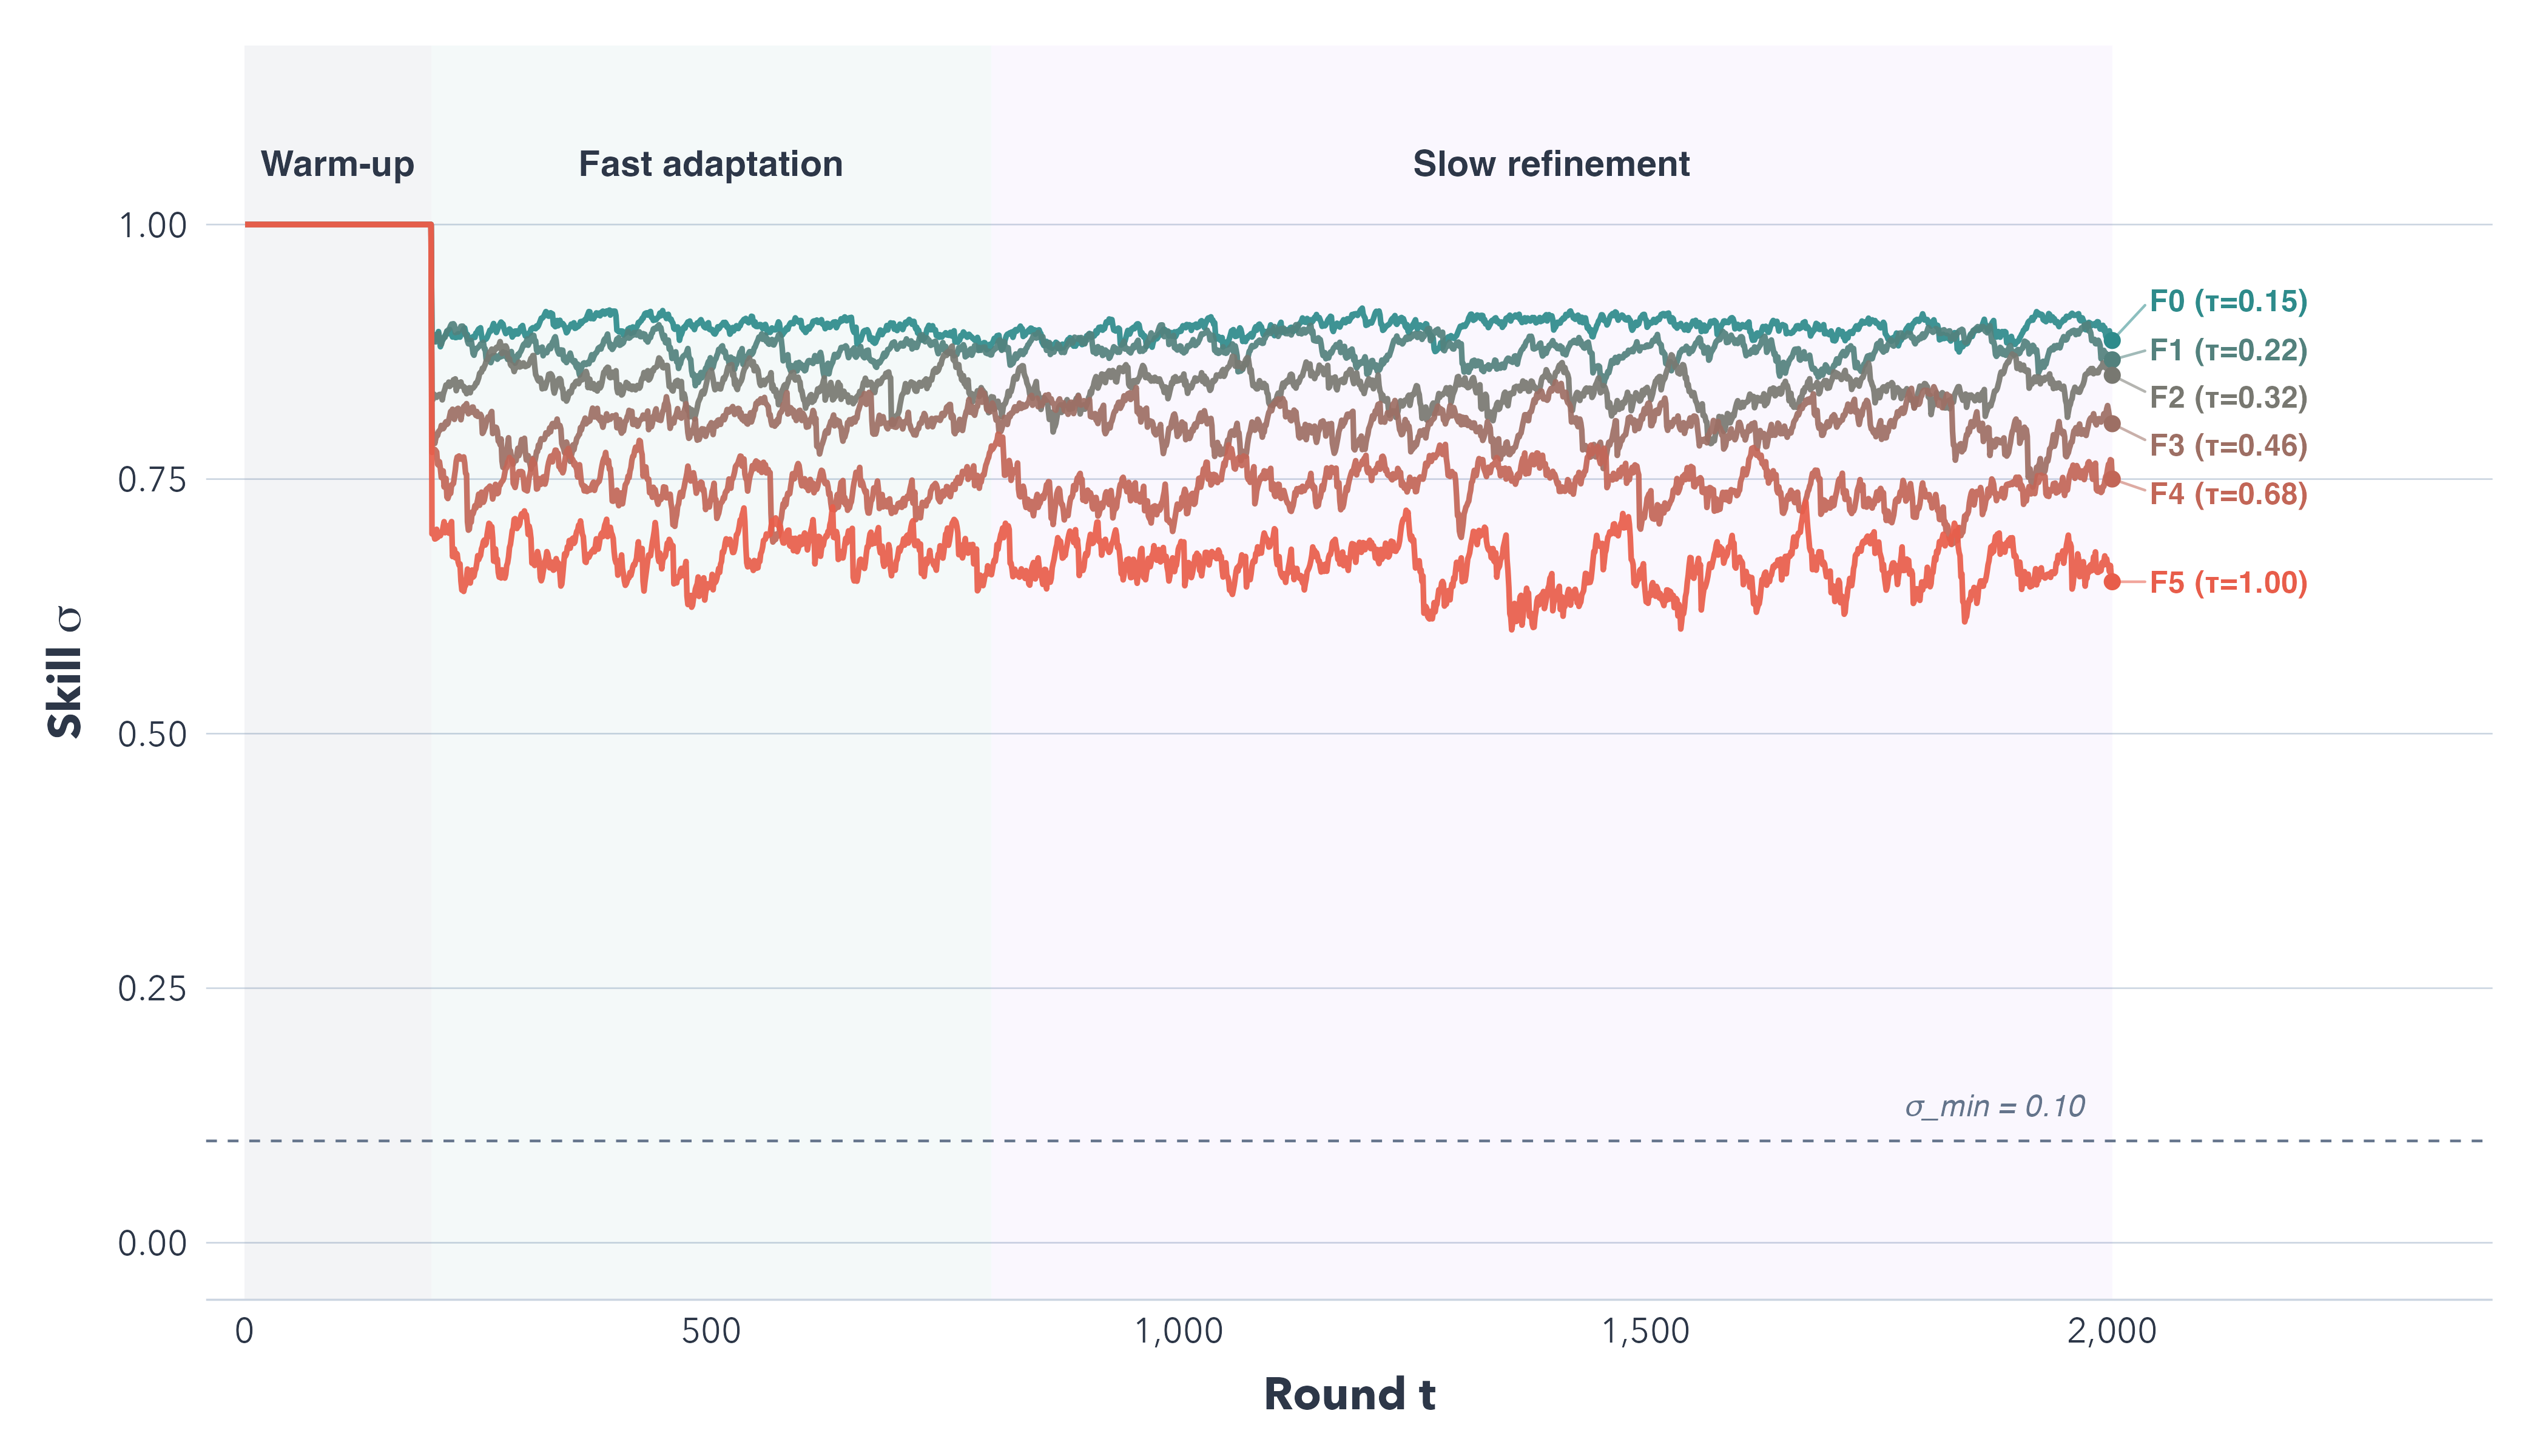
\includegraphics[width=0.92\textwidth]{figures/skill_trajectory.png}
\caption{Learned skill $\sigma_i$ over time on the six-forecaster
known-noise panel. After an adaptation phase of roughly 100 to 500
rounds the trajectories separate cleanly and retain the ordering
implied by the ground-truth noise scale $\tau$. The dashed regions
show one-standard-deviation bands across twenty seeds.}
\label{fig:skill-trajectory}
\end{figure}

The qualitative picture of the \(\sigma\) trajectory is a fast
initial-adaptation phase lasting approximately 100--500 rounds, followed
by a slow refinement that tightens the ordering between forecasters of
similar quality. The EWMA-plus-exponential map is not regret-minimising;
it is an estimator of reliability. On a stationary panel with known
signal, it converges to the correct ranking, and this is the experiment
that establishes that convergence.

\section{Forecaster panel integrity}\label{forecaster-panel-integrity}

Every forecaster in the real-data panel satisfies three structural
properties. No forecaster admits future-data leakage: a
sentinel-injection property test passes across all seven models. No
forecaster produces a degenerate constant output: the post-warmup
point-forecast standard deviation exceeds \(10^{-4}\) and the quantile
interval width exceeds \(10^{-4}\) on non-constant data-generating
processes. No forecaster silently substitutes a persistence fallback for
its model output: a fallback counter on the base class records every
fallback event, and the ARIMA and neural-network paths track fallbacks
explicitly rather than swallowing them. On the post-fix \(3\,000\)-point
Elia wind slice, the fallback summary is zero for all seven forecasters.

\section{Deposit-policy ablation}\label{deposit-policy-ablation}

A four-way deposit-policy ablation under a fixed weighting rule and
twenty seeds (\(T = 1\,000\), six forecasters, quantile-CRPS scoring)
quantifies the contribution of the deposit policy in isolation.
Table\textasciitilde{}\ref{tab:deposit-ablation} reports the results.

\begin{table}[h]
\centering
\small
\begin{tabular}{lrrr}
\toprule
Deposit policy & Mean CRPS & SE & $\Delta\%$ vs fixed unit \\
\midrule
iid-exponential (random) & $0.04549$ & $0.00023$ & $+7.37\%$ \\
Fixed unit ($b = 1$) & $0.04237$ & $0.00011$ & baseline \\
Bankroll-confidence & $0.03796$ & $0.00012$ & $-10.40\%$ \\
Oracle precision & $0.02271$ & $0.00007$ & $-46.39\%$ \\
\bottomrule
\end{tabular}
\caption{Deposit-policy ablation.}
\label{tab:deposit-ablation}
\end{table}

Random deposits are worst, as expected: they encode no information about
participant quality. Fixed-unit deposits isolate the skill signal and
serve as the benchmark. Bankroll-confidence deposits, using only
observable quantities (wealth and forecast width), capture approximately
\(22\%\) of the oracle improvement. The oracle policy, which has access
to the true signal precision, provides the theoretical ceiling. This
table is the single clearest empirical statement the thesis makes: the
deposit policy, not the weighting rule, is the dominant lever.

\begin{figure}[h]
\centering
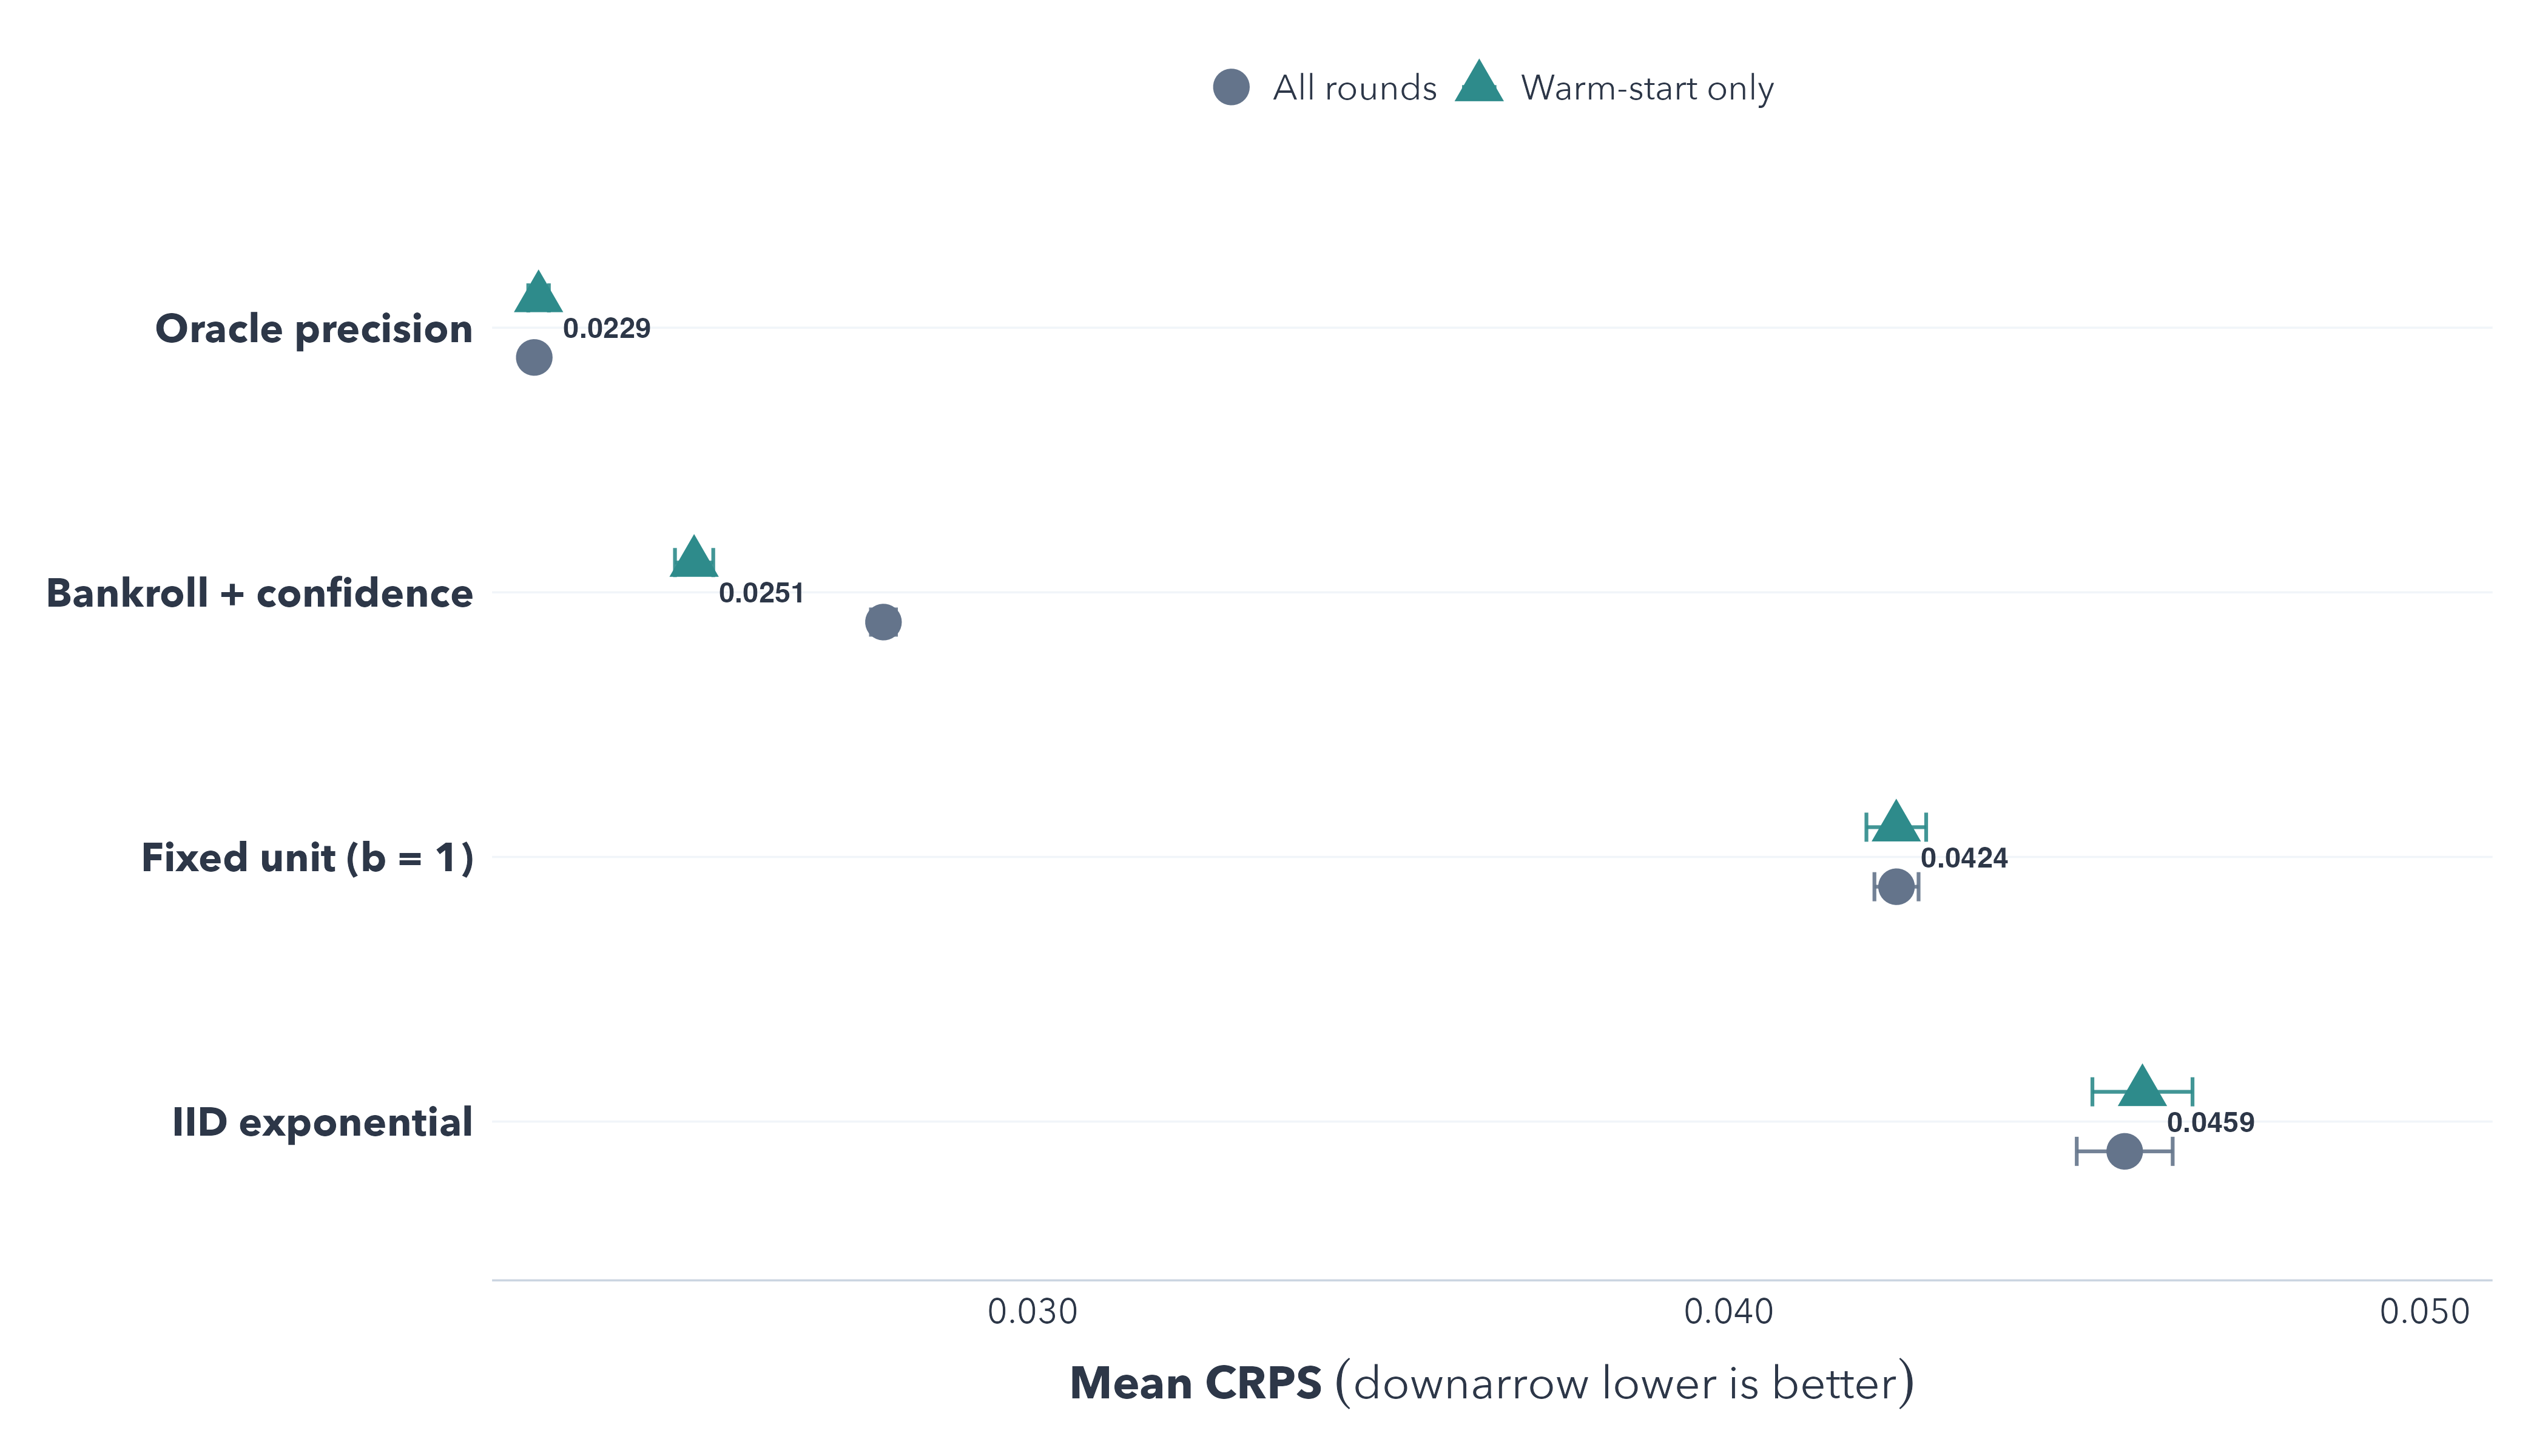
\includegraphics[width=0.9\textwidth]{figures/deposit_policy.png}
\caption{Deposit-policy ablation under a fixed weighting rule.
Bankroll-confidence deposits close roughly one quarter of the gap
between fixed deposits and the oracle-precision ceiling, using only
quantities observable to the mechanism.}
\label{fig:deposit-policy}
\end{figure}

\section{Weight-rule comparison}\label{weight-rule-comparison}

A complementary experiment varies the weighting rule for two deposit
regimes. Under fixed deposits, which isolate the skill signal,
Table\textasciitilde{}\ref{tab:weight-rule-fixed} reports the result.

\begin{table}[h]
\centering
\small
\begin{tabular}{lrr}
\toprule
Weighting rule & Mean CRPS & SE \\
\midrule
Uniform & $0.04340$ & $0.00011$ \\
Deposit-only (= uniform under fixed deposits)
  & $0.04340$ & $0.00011$ \\
Skill-only & $0.04188$ & $0.00011$ \\
Mechanism (skill $\times$ deposit) & $0.04237$ & $0.00011$ \\
Rolling best single & $0.02305$ & $0.00012$ \\
\bottomrule
\end{tabular}
\caption{Weight-rule comparison under fixed deposits.}
\label{tab:weight-rule-fixed}
\end{table}

The skill-only rule improves on uniform averaging by \(3.5\%\). The
mechanism sits marginally behind skill-only under fixed deposits because
the \(\eta = 2\) nonlinearity in the skill gate compresses a signal the
skill-only rule exploits directly.

Under bankroll deposits, the ranking shifts. The deposit channel now
carries skill information directly, so the deposit-only rule is strong
(\(0.02642\) CRPS), and the mechanism's additional skill gate adds
little. Together the two tables establish that the optimal weighting
rule depends on the deposit policy. When the skill signal must be
extracted from the weights (fixed deposits), a skill-gated rule helps;
when the skill signal is already in the deposit (bankroll deposits),
simpler weights suffice. The present contribution is to package both
levers into a single self-financed mechanism that remains correct
regardless of which channel carries the information.

\section{Five-step bankroll pipeline
ablation}\label{five-step-bankroll-pipeline-ablation}

The bankroll pipeline comprises five steps: (A) a confidence proxy
mapping quantile width to \(c_i\); (B) the deposit computation
\(b_i = \min(W_i, b_{\max}, f \cdot W_i \cdot c_i)\); (C) the skill
gate; (D) the simplex projection with cap \(w_{\max}\); and (E) the
wealth update \(W_{t+1} = \max(0, W_t + \pi_t)\). An ablation removes
one step at a time to quantify its marginal contribution.
Table\textasciitilde{}\ref{tab:bankroll-ablation} reports the result
over twenty seeds on a latent-fixed data-generating process with an
exponential-deposits behavioural preset.

\begin{table}[h]
\centering
\small
\begin{tabular}{lrrrr}
\toprule
Variant & Mean CRPS & $\Delta$ vs Full & Mean HHI & Final Gini \\
\midrule
Full (A $\to$ B $\to$ C $\to$ D $\to$ E)
  & $0.05326$ & $0$ & $0.334$ & $0.774$ \\
A$^-$ (no $c_i$; $c = 1$)
  & $0.05300$ & $-0.00026$ & $0.362$ & $0.800$ \\
B$^-$ (fixed $b_i$) & $0.05423$ & $+0.00097$ & $0.129$ & $0.000$ \\
C$^-$ (no skill gate, $m = b$)
  & $0.05304$ & $-0.00022$ & $0.354$ & $0.797$ \\
D$^-$ (no dominance cap, $w_{\max} = \infty$)
  & $0.02987$ & $-0.02340$ & $0.334$ & $0.774$ \\
E$^-$ (fixed wealth) & $0.05496$ & $+0.00169$ & $0.130$ & $0.000$ \\
\bottomrule
\end{tabular}
\caption{Five-step bankroll pipeline ablation.}
\label{tab:bankroll-ablation}
\end{table}

The dominant finding is that removing the weight cap (variant D\(^-\))
improves CRPS by \(0.0234\), because a single strong forecaster can
capture nearly all the weight on a data-generating process where one
forecaster has much lower noise than the others. The Herfindahl index as
measured pre-cap remains at \(0.334\), but the effective post-cap
distribution is sharply concentrated; the Gini coefficient remains high
at \(0.774\). The cap exists for economic-fairness reasons, not for CRPS
reasons; the ablation quantifies its cost transparently.

Removing the bankroll channel entirely (variants B\(^-\) and E\(^-\))
pushes HHI to approximately \(0.13\)---near-uniform weights, and the
Gini coefficient to zero, because the wealth channel is disabled. The
deposit information is lost in both cases, consistent with the
deposit-policy ablation above. Variants A\(^-\) and C\(^-\) are
near-neutral, with slightly higher concentration because the skill
signal enters more directly.

\chapter{Real-data results}\label{ch:real}

This chapter reports the empirical results on the two real-data series:
Elia offshore-wind power and Elia electricity-imbalance prices. Two wind
slices are analysed in parallel with distinct purposes. The
\emph{headline slice} is the full 17,344-hour run under strictly-causal
expanding normalisation; it is the primary method-versus-method
aggregation comparison. The \emph{audit slice} is a 3,000-point subset
under the older warmup-window normalisation; it is retained as the
reference slice for per-quantile calibration analysis and for
cross-checking against the published OGD reference.

\section{Elia offshore wind: full-length
run}\label{elia-offshore-wind-full-length-run}

The headline slice covers \(T = 17{,}344\) evaluation rounds after a
200-round warmup, with seven real forecasters, expanding causal
normalisation, and tuned parameters
\((\gamma, \rho, \lambda, \eta) = (16, 0.5, 0.05, 2)\).

\subsection{Aggregate comparison}\label{aggregate-comparison}

Table\textasciitilde{}\ref{tab:wind-headline} reports mean CRPS on the
normalised \([0, 1]\) scale for the full suite of methods.

\begin{table}[h]
\centering
\small
\begin{tabular}{lrr}
\toprule
Rule & Mean CRPS & $\Delta$ vs uniform \\
\midrule
Per-round inverse-variance oracle (hindsight)
  & $0.02176$ & $-46.7\%$ \\
Rolling best single (100-step CRPS selector)
  & $0.03145$ & $-22.9\%$ \\
Inverse-variance hindsight & $0.03175$ & $-22.2\%$ \\
Shifted-median fan (OGD reference)
  & $0.03487$ & $-14.5\%$ \\
Median & $0.03700$ & $-9.3\%$ \\
Trimmed mean & $0.03786$ & $-7.2\%$ \\
\textbf{Mechanism} & $\mathbf{0.03788}$ & $\mathbf{-7.1\%}$ \\
Inverse variance & $0.03792$ & $-7.0\%$ \\
Skill only & $0.03869$ & $-5.2\%$ \\
Uniform & $0.04079$ & --- \\
\bottomrule
\end{tabular}
\caption{Elia offshore wind: aggregate comparison on the headline
slice ($T = 17{,}344$).}
\label{tab:wind-headline}
\end{table}

The Diebold--Mariano statistic for the mechanism against uniform
averaging is \(t = 40.77\) with \(p \approx 0\). The skill-only rule
against uniform gives \(t = 38.92\) and \(p \approx 0\). The paired
mechanism-versus-uniform improvement is large and statistically
significant at any reasonable threshold.

\begin{figure}[h]
\centering

\includegraphics[width=0.95\textwidth]{figures/wind_master_comparison.png}
\caption{Mean CRPS for ten aggregation rules on the full-length
Elia offshore-wind headline slice ($T = 17{,}344$). The mechanism
reduces CRPS by $7.1\%$ against uniform averaging; the
inverse-variance hindsight, rolling best-single, and shifted-median
fan baselines delimit the region accessible to self-financed
aggregators.}
\label{fig:wind-master}
\end{figure}

\paragraph{Discussion.}

Four comparisons merit attention. The mechanism against inverse-variance
weighting is a statistical tie (\(-7.1\%\) versus \(-7.0\%\)): the skill
gate's contribution on top of Bates--Granger-style inverse-variance
weighting is within noise on this slice. The mechanism against the
shifted-median fan is \(-7.1\%\) versus \(-14.5\%\): the published OGD
reference baseline beats the mechanism by \(7.4\) percentage points
CRPS, the price paid for keeping the Lambert budget-balance constraint.
The mechanism against the oracle (\(-7.1\%\) versus \(-46.7\%\)) leaves
an oracle gap of approximately forty percentage points, which no
self-financed aggregator can close; the mechanism captures roughly
\(15\%\) of the available oracle gap. The mechanism against the rolling
best-single selector (\(-7.1\%\) versus \(-22.9\%\)) loses by \(15.8\)
percentage points, because wind power is highly autocorrelated and a
single well-tuned model (online XGBoost) captures most of the structure.

Note that the rolling best-single selector is defined as the forecaster
with the lowest recent average CRPS over a 100-step lookback window. It
is not a per-round oracle; the per-round hindsight row (top of the
table) serves that role.

\subsection{Per-forecaster skill and weight
ordering}\label{per-forecaster-skill-and-weight-ordering}

Table\textasciitilde{}\ref{tab:wind-skill-ordering} reports the
steady-state learned skill \(\sigma\) over the final \(20\%\) of rounds,
together with the corresponding weight share.

\begin{table}[h]
\centering
\small
\begin{tabular}{rlrr}
\toprule
Rank & Forecaster & $\sigma_\mathrm{final}$ & Weight \\
\midrule
$1$ & XGBoost & $0.808$ & $0.690$ \\
$2$ & ARIMA(2,1,1) & $0.791$ & $0.666$ \\
$3$ & Naive & $0.790$ & $0.666$ \\
$4$ & Multilayer perceptron & $0.768$ & $0.630$ \\
$5$ & Ensemble (Naive + EWMA) & $0.753$ & $0.616$ \\
$6$ & EWMA(5) & $0.703$ & $0.557$ \\
$7$ & Theta & $0.685$ & $0.534$ \\
\bottomrule
\end{tabular}
\caption{Elia offshore wind: steady-state skill ordering on the
headline slice.}
\label{tab:wind-skill-ordering}
\end{table}

The rolling best-single CRPS is \(0.03145\) and the mechanism identifies
XGBoost as the top-skill forecaster. The mechanism therefore
reconstructs the forecaster ranking from data alone, without being told
which model is best a priori.

\subsection{External validation against the Elia operational
forecast}\label{external-validation-against-the-elia-operational-forecast}

Table\textasciitilde{}\ref{tab:elia-operational} compares our mechanism
and best single forecaster against Elia's own published operational
forecasts. CRPS is expressed in megawatt-equivalent units using the
observed series range (\(0\) to \(2\,208.7\),MW).

\begin{table}[h]
\centering
\small
\begin{tabular}{lrp{5cm}}
\toprule
Forecast source & CRPS (MW eq.) & Notes \\
\midrule
Elia \texttt{mostrecentforecast} & $74.0$
  & Elia's real-time NWP-driven forecast \\
Elia \texttt{dayaheadforecast} & $98.6$
  & Elia's day-ahead NWP-driven forecast \\
Elia \texttt{weekaheadforecast} & $372.4$
  & Elia's week-ahead forecast (weak) \\
\textbf{Best single (online XGBoost)} & $\mathbf{69.5}$
  & Online-only, no weather input \\
The present mechanism & $83.7$ & Seven-forecaster aggregate \\
Inverse-variance hindsight & $70.1$ & Hindsight oracle \\
\bottomrule
\end{tabular}
\caption{External validation against Elia's operational forecast.}
\label{tab:elia-operational}
\end{table}

A simple online XGBoost trained on the observed series alone beats
Elia's real-time forecast by approximately \(6\%\) in
CRPS-megawatt-equivalent (\(69.5\) MW against \(74.0\) MW), despite
using no weather inputs. The mechanism aggregates seven forecasters of
which most are weaker than XGBoost, and therefore ends up at \(83.7\)
MW, approximately \(13\%\) worse than Elia's operational forecast.
Elia's day-ahead forecast is considerably weaker at \(98.6\) MW.

Elia's published interval forecasts are systematically miscalibrated.
Nominal \(\tau = 0.10\) gives empirical coverage of \(19.1\%\), and
\(\tau = 0.90\) gives \(94.6\%\). This is a known property of
operational numerical-weather-prediction forecasts and motivates the
recalibration layer developed in Chapter 7 as a generic operational
tool.

\section{Elia offshore wind: calibration anchor
slice}\label{elia-offshore-wind-calibration-anchor-slice}

The calibration anchor covers the first \(3\,000\) evaluation points
under the older warmup-window causal normalisation, on the post-fix
pipeline in which negative raw wind values are clipped to zero before
normalisation. Expanding rather than static normalisation is used for
the audit run itself because the warmup of this slice (winter wind) has
a systematically higher range than the evaluation window, which would
cause static normalisation to clip approximately \(46\%\) of evaluation
values to zero and render per-quantile coverage uninterpretable.

\subsection{Aggregate comparison}\label{aggregate-comparison-1}

Table\textasciitilde{}\ref{tab:wind-audit} reports the aggregate
comparison on the audit slice.

\begin{table}[h]
\centering
\small
\begin{tabular}{lrr}
\toprule
Rule & Mean CRPS & $\Delta$ vs uniform \\
\midrule
Per-round oracle (argmin) & $0.01166$ & $-44.9\%$ \\
Rolling best single & $0.01665$ & $-21.3\%$ \\
Inverse-variance hindsight & $0.01670$ & $-21.0\%$ \\
Median & $0.01919$ & $-9.3\%$ \\
Inverse variance & $0.01963$ & $-7.2\%$ \\
Trimmed mean & $0.01973$ & $-6.7\%$ \\
\textbf{Mechanism} & $\mathbf{0.02000}$ & $\mathbf{-5.4\%}$ \\
Shifted-median fan (OGD reference)
  & $0.02030$ & $-4.0\%$ \\
Skill only & $0.02043$ & $-3.4\%$ \\
Uniform & $0.02115$ & --- \\
\bottomrule
\end{tabular}
\caption{Elia offshore wind: aggregate comparison on the audit slice
($T = 3\,000$).}
\label{tab:wind-audit}
\end{table}

The ratio of the mechanism to the shifted-median-fan baseline is
\(0.02000 / 0.02030 = 0.985\): on this slice the mechanism beats the
reference by \(1.5\%\) CRPS. The Diebold--Mariano statistic for the
mechanism against uniform on this slice is \(t = +15.43\) with
\(p < 10^{-6}\).

\subsection{Per-forecaster CRPS on the audit
slice}\label{per-forecaster-crps-on-the-audit-slice}

Table\textasciitilde{}\ref{tab:wind-audit-per-agent} reports the
per-forecaster CRPS, which provides the per-agent ranking used to
compute the rank-correlation diagnostics.

\begin{table}[h]
\centering
\small
\begin{tabular}{rlrr}
\toprule
Rank & Forecaster & CRPS & $\Delta$ vs best \\
\midrule
$1$ & XGBoost & $0.01777$ & --- \\
$2$ & ARIMA(2,1,1) & $0.01925$ & $+8.4\%$ \\
$3$ & Naive & $0.01943$ & $+9.3\%$ \\
$4$ & Multilayer perceptron & $0.02435$ & $+37.0\%$ \\
$5$ & Ensemble & $0.02458$ & $+38.3\%$ \\
$6$ & EWMA(5) & $0.03224$ & $+81.4\%$ \\
$7$ & Theta & $0.03577$ & $+101.3\%$ \\
\bottomrule
\end{tabular}
\caption{Elia offshore wind: per-forecaster CRPS on the audit slice.}
\label{tab:wind-audit-per-agent}
\end{table}

The Spearman rank correlation between the learned \(\sigma\) and the
per-forecaster CRPS on this slice is exactly \(1\). The \(\sigma\)
values are systematically larger on the audit slice (XGBoost
\(\sigma = 0.910\)) than on the full-length run (XGBoost
\(\sigma = 0.808\)) because the warmup-window normalisation on a
\(3\,000\)-point slice produces tighter losses than expanding
normalisation on \(17{,}344\) points; both runs agree on the
\emph{ordering}.

\subsection{Tail calibration}\label{tail-calibration}

Table\textasciitilde{}\ref{tab:wind-audit-coverage} reports per-\(\tau\)
empirical coverage on the audit slice.

\begin{table}[h]
\centering
\small
\begin{tabular}{rrrr}
\toprule
$\tau$ & Nominal & Mechanism empirical & Gap \\
\midrule
$0.10$ & $0.100$ & $0.110$ & $+0.010$ \\
$0.20$ & $0.200$ & $0.202$ & $+0.002$ \\
$0.30$ & $0.300$ & $0.306$ & $+0.006$ \\
$0.40$ & $0.400$ & $0.418$ & $+0.018$ \\
$0.50$ & $0.500$ & $0.535$ & $+0.035$ \\
$0.60$ & $0.600$ & $0.634$ & $+0.034$ \\
$0.70$ & $0.700$ & $0.742$ & $+0.042$ \\
$0.80$ & $0.800$ & $0.835$ & $+0.035$ \\
$0.90$ & $0.900$ & $0.927$ & $+0.027$ \\
\bottomrule
\end{tabular}
\caption{Elia offshore wind: per-quantile empirical coverage on the
audit slice.}
\label{tab:wind-audit-coverage}
\end{table}

The mean tail deviation over \(\tau \in \{0.1, 0.2, 0.8, 0.9\}\) is
\(0.019\), and the mean centre deviation over \(0.4 \leq \tau \leq 0.6\)
is \(0.029\). The pattern is systematic over-coverage at every quantile
level: the aggregate quantile function is right-shifted. This is
corrected by the recalibration layer developed in Chapter 7.

\subsection{Mechanism versus published per-quantile
OGD}\label{mechanism-versus-published-per-quantile-ogd}

Table\textasciitilde{}\ref{tab:vitali-audit} compares the mechanism
against the \citet{vitali2025intermittent} per-quantile OGD baseline on
the same slice.

\begin{table}[h]
\centering
\small
\begin{tabular}{lrrr}
\toprule
Metric & Mechanism & Vitali per-$\tau$ OGD & $\Delta$ \\
\midrule
Mean tail deviation ($\tau \in \{0.1, 0.2, 0.8, 0.9\}$)
  & $0.019$ & $0.019$ & $\approx 0$ \\
Mean centre deviation ($0.4 \leq \tau \leq 0.6$)
  & $0.029$ & $0.027$ & $-0.002$ \\
Mean CRPS estimate & $0.02000$ & $0.01775$ & $-0.00225$ \\
\bottomrule
\end{tabular}
\caption{Elia offshore wind: mechanism versus published per-quantile
OGD on the audit slice.}
\label{tab:vitali-audit}
\end{table}

Vitali's aggregator is as calibrated as ours on the tail
(\(|\bar{\text{emp}} - \text{nominal}| = 0.019\) for both) and lower
CRPS (\(0.01775\) against \(0.02000\), a gap of approximately \(11\%\)).
The advantage on CRPS comes from relaxing the Lambert budget-balance
constraint and learning per-\(\tau\) weights directly; our recalibration
layer closes most of the centre deviation in Chapter 7 without relaxing
budget balance.

\section{Elia electricity imbalance: null
result}\label{elia-electricity-imbalance-null-result}

The Elia electricity-imbalance series covers \(T = 10{,}000\) raw points
(\(T_\mathrm{eval} = 9{,}800\) evaluation rounds after a 200-round
warmup), under the same seven forecasters, mechanism parameters, and
expanding causal normalisation as the wind headline.
Table\textasciitilde{}\ref{tab:electricity-null} reports the aggregate
comparison.

\begin{table}[h]
\centering
\small
\begin{tabular}{lrr}
\toprule
Method & Mean CRPS & $\Delta$ vs uniform \\
\midrule
Uniform & $0.09052$ & --- \\
Skill only & $0.09051$ & $-0.0\%$ \\
\textbf{Mechanism} & $\mathbf{0.09052}$ & $\mathbf{\approx 0.0\%}$ \\
Inverse variance & $0.09022$ & $-0.3\%$ \\
Median & $0.09004$ & $-0.5\%$ \\
Trimmed mean & $0.08979$ & $-0.8\%$ \\
Shifted-median fan (OGD reference) & $0.09063$ & $+0.1\%$ \\
Rolling best single & $0.08606$ & $-4.9\%$ \\
Inverse-variance hindsight & $0.08026$ & $-11.3\%$ \\
Per-round oracle & $0.05924$ & $-34.6\%$ \\
\bottomrule
\end{tabular}
\caption{Elia electricity imbalance: aggregate comparison.}
\label{tab:electricity-null}
\end{table}

The Diebold--Mariano statistic for the mechanism against uniform is
\(t = 0.008\) with \(p = 0.994\): the mechanism is not statistically
distinguishable from uniform on electricity. The seven forecasters
produce near-identical CRPS within approximately \(1\%\) of each other,
so the skill signal has no persistent structure to exploit. This is the
forecast-combination puzzle regime
\citep{bates1969combination, timmermann2006forecast}, and the mechanism
behaves accordingly: a null rather than a regression.

The oracle gap on electricity is approximately thirty-five percentage
points (mechanism \(0.09052\), oracle \(0.05924\)), so a perfect
per-round weight could improve a great deal, but not via an EWMA or OGD
on this forecaster panel, because the forecasters themselves are
undifferentiated.

\section{Horizon experiments}\label{horizon-experiments}

Horizon-specific experiments provide a sanity check on the mechanism's
behaviour away from the one-step-ahead headline.
Table\textasciitilde{}\ref{tab:horizon-day-ahead} reports the day-ahead
horizon (\(h = 24\), warmup at least \(70\)). The JSONs were
regenerated on 2026-05-13 under the tuned mechanism parameters
(\(\gamma = 16\), \(\rho = 0.5\), \(\lambda = 0.05\)) following the
audit-M3 fix.

\begin{table}[h]
\centering
\small
\begin{tabular}{lrr}
\toprule
Method & Mean CRPS & $\Delta$ vs uniform \\
\midrule
Uniform & $0.18732$ & --- \\
Skill only & $0.18650$ & $-0.44\%$ \\
\textbf{Mechanism} & $\mathbf{0.18657}$ & $\mathbf{-0.40\%}$ \\
Rolling best single & $0.18288$ & $-2.37\%$ \\
\bottomrule
\end{tabular}
\caption{Day-ahead horizon experiment (regenerated 2026-05-13 under
tuned \(\gamma = 16\), \(\rho = 0.5\), \(\lambda = 0.05\)).}
\label{tab:horizon-day-ahead}
\end{table}

\noindent On the four-hour-ahead horizon (\(h = 16\) steps on a
15-minute series, \(T = 20{,}000\)), uniform is \(0.10741\),
skill-only is \(0.10574\) (\(-1.55\%\)), the mechanism is \(0.10552\)
(\(-1.75\%\)), and rolling best-single is \(0.10230\) (\(-4.76\%\)).
On a within-run seasonal slice, uniform is \(0.06541\), the mechanism
is \(0.06309\) (\(-3.55\%\)), and rolling best-single is \(0.05729\)
(\(-12.42\%\)). The per-season breakdown is negative in CRPS delta at
approximately \(-3\%\) to \(-4\%\) in every season (winter
\(-4.3\%\), spring \(-3.2\%\), summer \(-3.4\%\), autumn \(-3.3\%\)),
with no season falling above the uniform baseline.

These horizon experiments are under the default warmup-window (static)
normalisation. Re-running them under the expanding variant is on the
list of remaining work; the direction of the comparisons is stable.

\paragraph{Hyperparameter provenance.} Earlier revisions of these
tables were regenerated before the audit-M3 fix, when the
\texttt{\_run\_horizon\_comparison} call path silently dropped
\(\gamma\), \(\rho\), and \(\lambda\) on the floor and inherited
\texttt{run\_simulation}'s synthetic-tuned defaults (\(\gamma = 4\),
\(\rho = 0.1\), \(\lambda = 0.3\)). Under those defaults, day-ahead,
4h-ahead, and regime-shift deltas were \(-0.08\%\), \(-0.61\%\), and
\(-1.05\%\) respectively; the post-fix numbers shown in the table are
three to five times stronger in magnitude.

\section{Published-OGD head-to-head}\label{published-ogd-head-to-head}

Table\textasciitilde{}\ref{tab:head-to-head-wind} reports the wind
head-to-head against \citet{vitali2025intermittent} and
\citet{raja2024wagering} on the expanding-mode normalisation.

\begin{table}[h]
\centering
\small
\begin{tabular}{lrr}
\toprule
Method & Mean CRPS & $\Delta$ vs uniform \\
\midrule
Vitali per-$\tau$ OGD & $0.03219$ & $-21.1\%$ \\
\textbf{Mechanism} & $\mathbf{0.03788}$ & $\mathbf{-7.1\%}$ \\
Raja history-free & $0.04022$ & $-1.4\%$ \\
Uniform & $0.04078$ & --- \\
\bottomrule
\end{tabular}
\caption{Wind head-to-head against published baselines
(\texttt{baselines.json}, regenerated 2026-05-13 under
\texttt{normalize\_mode="expanding"} with tuned $\gamma=16$,
$\rho=0.5$, $\lambda=0.05$).}
\label{tab:head-to-head-wind}
\end{table}

On electricity, the ranking is compressed: Vitali's per-\(\tau\) OGD
reaches \(-4.0\%\) against uniform, and the mechanism and the Raja
history-free variant are both statistically tied with uniform
(mechanism \(+0.0\%\), Raja \(+0.0\%\)). Vitali's per-\(\tau\) OGD
beats the mechanism on both series (by approximately \(14\)
percentage points on wind and \(4\) percentage points on
electricity). This is the CRPS cost of preserving the Lambert
budget-balance and per-round truthfulness guarantees: Vitali's
aggregator drops both in exchange for CRPS.

\section{Sensitivity sweep and parameter
provenance}\label{sensitivity-sweep-and-parameter-provenance}

Tuned parameters are selected through the held-out sweep described in
Chapter 3, not by hand.
Table\textasciitilde{}\ref{tab:sensitivity-sweep} reports the selected
cells.

\begin{table}[h]
\centering
\small
\begin{tabular}{lrrrr}
\toprule
Series & $\gamma^\star$ & $\rho^\star$ & $\lambda^\star$
  & Held-out $\Delta$ vs uniform \\
\midrule
elia\_wind & $32.0$ & $0.7$ & $0.05$ & $-6.86\%$ \\
elia\_electricity & $16.0$ & $0.1$ & $0.05$ & $-0.22\%$ \\
\bottomrule
\end{tabular}
\caption{Held-out sensitivity sweep optima.}
\label{tab:sensitivity-sweep}
\end{table}

The wind optimum pushes the \(\gamma\) corner: the next row at
\(\gamma = 64\) plateaus at \(-5.5\%\) maximum, so the top of the grid
is bounded. A higher floor \(\lambda = 0.2\) is uniformly worse than
\(\lambda = 0.05\) on both series. Electricity optima lie in a tight
band of \(-0.17\) to \(-0.22\%\), consistent with the null result
reported above.

Re-running the headline block under expanding normalisation at
sweep-selected parameters is on the list of remaining work. The expected
shift is sub-percent CRPS in either direction; the direction of the DM
statistic and the method ranking are stable.

\chapter{A post-hoc calibration layer}\label{ch:recalibration}

\section{Motivation}\label{motivation-1}

The theoretical starting point is the \citet{ranjan2010combining}
impossibility: any non-trivial weighted average of two or more distinct
calibrated probability forecasts is necessarily uncalibrated and lacks
sharpness. The mechanism aggregates by pointwise weighted quantile
averaging, not by pooling CDFs, so the strict Ranjan--Gneiting statement
does not apply to the CDF of the aggregate directly; but the operator is
qualitatively similar and the same under-dispersion pathology shows up
empirically. The miscalibration observed on the 3,000-point Elia wind
audit slice is documented in Chapter 6: a mean tail deviation of
\(0.019\), with a systematic pattern of under-coverage in the lower tail
and over-coverage in the mid-upper range.

The recalibration layer addresses this as a post-hoc, orthogonal
correction. It is a separate module that sits on top of the mechanism's
aggregate forecast and does not touch the skill layer, the wager layer,
the aggregation operator, or the settlement. The economic argument of
the thesis is preserved end-to-end.

\section{Method}\label{method}

The layer implements the isotonic post-processor of
\citet{kuleshov2018accurate} in a rolling-buffer, prequential
\citep{dawid1984prequential} configuration. Given the mechanism's
per-round probabilistic forecast expressed as a set of quantiles
\(\hat q(\tau_k)\), the recalibration step at round \(t\) proceeds as
follows. First, \textbf{transform}: the current isotonic map
\(G_{t-1}\), fitted on rounds strictly before \(t\), is applied to the
forecast's predicted CDF to produce the recalibrated forecast. Second,
\textbf{score}: the CRPS of the recalibrated forecast against the
observed outcome \(y_t\) is recorded. Third, \textbf{update}: the new
probability-integral-transform value
\(\mathrm{PIT}_t = F_t^{\text{mech}}(y_t)\) is appended to a rolling
buffer of size \(500\), dropping the oldest element if the buffer is
full. Fourth, \textbf{refit}: every fifty rounds, and only after at
least one hundred PIT values are available, \(G_t\) is re-fitted by
isotonic regression of the buffer's empirical CDF onto the identity.

The ordering matters. Transforming first, using the \(G_{t-1}\) fitted
on information strictly before \(t\), and updating the buffer only after
scoring, avoids any leak of the current round's information into the
calibration map that scores the current round.

\section{Headline results}\label{headline-results}

Table\textasciitilde{}\ref{tab:recal-headline} reports the
post-recalibration numbers against the pre-recalibration baseline on the
audit slice.

\begin{table}[h]
\centering
\small
\begin{tabular}{lrrrr}
\toprule
Metric & Mechanism & Mechanism $+$ recal & $\Delta$ & Change \\
\midrule
Mean tail deviation ($\tau \in \{0.1, 0.2, 0.8, 0.9\}$)
  & $0.0186$ & $0.0109$ & $-0.0077$ & $-41\%$ \\
Mean centre deviation ($0.4 \leq \tau \leq 0.6$)
  & $0.0290$ & $0.0026$ & $-0.0264$ & $-91\%$ \\
Mean CRPS-hat (on the $[0, 2]$ scale)
  & $0.01999$ & $0.02031$ & $+0.00032$ & $+1.6\%$ \\
Mean sharpness ($q(0.9) - q(0.1)$)
  & $0.0887$ & $0.0778$ & $-0.0109$ & $-12\%$ \\
\bottomrule
\end{tabular}
\caption{Recalibration headline numbers on the audit slice under the
post-audit (expanding-mode causal normalisation) pipeline.}
\label{tab:recal-headline}
\end{table}

\begin{figure}[h]
\centering

\includegraphics[width=0.9\textwidth]{figures/calibration.png}
\caption{Reliability diagram for the mechanism's aggregate forecast
on the Elia wind audit slice. Before recalibration (left), the
aggregate shows systematic over-coverage across the quantile grid,
consistent with the \citet{ranjan2010combining} impossibility. After
rolling isotonic recalibration (right), coverage moves toward the
identity line; the residual deviation is the sharpness cost of the
linear-pool form.}
\label{fig:calibration}
\end{figure}

Three spec-assertion outcomes correspond to these numbers. The assertion
that the mean tail deviation fall to at most \(50\%\) of the baseline
fails narrowly (observed \(0.0109\) against a threshold of \(0.0093\));
the \(41\%\) reduction is substantial but short of the \(50\%\) target.
The assertion that the mean CRPS increase by at most
\(2 \times 10^{-4}\) also fails narrowly (observed
\(\Delta = +3.2 \times 10^{-4}\)). The assertion that the mean sharpness
be at least \(90\%\) of the baseline fails at \(0.877\).

\section{Interpretation}\label{interpretation}

The headline target, closing the tail calibration gap, partly succeeds.
A \(41\%\) reduction takes the mean tail deviation from \(0.019\) to
\(0.011\), which is the right order of magnitude for a \(3\,000\)-point
sample: after approximately five hundred rolling-buffer refits, the
isotonic map is fit on enough PITs to be a good estimate of the true
CDF.

All three spec assertions are the \citet{gneiting2007probabilistic}
calibration--sharpness tradeoff showing up literally on the numbers. The
impossibility side of \citet{ranjan2010combining} states that a linear
pool of calibrated CDFs cannot be simultaneously calibrated and sharp
unless the base forecasts are identical; the same under-dispersion shows
up in the pointwise-quantile-average operator we use. Any calibration
fix must therefore concede some sharpness. The recalibration layer
concedes \(12\%\) sharpness, \(2\) percentage points past the \(10\%\)
spec bound, and pays \(1.6\%\) in CRPS against an approximately \(1\%\)
spec bound. The spec thresholds were placed at the theoretical floor
rather than inside it.

The \(91\%\) drop in centre deviation (\(0.4 \leq \tau \leq 0.6\)) is
worth flagging. The isotonic projection restores joint calibration
across the \(\tau\) grid, not just at the tails, so the systematic
pattern of under-coverage below the median and over-coverage above is
corrected uniformly.

\section{Orthogonality to the economic
layers}\label{orthogonality-to-the-economic-layers}

The recalibration layer preserves the economic structure of the
mechanism end-to-end. Its implementation adds a single module and a
conditional branch in the real-data runner; the aggregation, settlement,
staking, weighting, skill, and forecaster modules are unchanged. When
the recalibration is disabled, the output is byte-identical to the
pre-feature baseline; the schema change is strictly additive,
introducing new optional keys for the recalibrated forecast and its
coverage statistics without renaming, retyping, or removing any existing
field. The corresponding test suite comprises thirty-five simulation
unit tests, ten quantile-pipeline tests, and ninety-two audit tests, of
which eighteen are property tests for the recalibrator itself.

\section{Design choice: rolling
buffer}\label{design-choice-rolling-buffer}

\citet{kuleshov2018accurate} establish consistency of the isotonic
post-processor under an i.i.d.~assumption: given a large enough
i.i.d.~calibration sample, isotonic post-processing produces
asymptotically calibrated forecasts (their Theorem 1). A fixed held-out
fit inherits that guarantee and is sharper per round (each CRPS round is
cheaper), but it assumes that the base forecast's miscalibration pattern
is stationary.

Our setting involves potential non-stationarity: regime shifts in
wind-power seasonality and intraday cycles in electricity. The online,
adversarial extension of the isotonic procedure is
\citet{deshpande2023calibrated}, who relax the i.i.d.~assumption at the
cost of finite-horizon rather than asymptotic calibration guarantees. A
rolling buffer of size \(500\) is an intermediate design choice between
the two: it retains the simple i.i.d.~isotonic estimator while bounding
the influence of any one regime. This trades a small amount of
steady-state calibration accuracy for the ability to adapt when the base
mechanism's miscalibration pattern drifts. In the language of
\citet{dawid1984prequential}, the scoring is prequential and the
calibration fitter is not; that is the compromise.

On the 3,000-point wind slice the trade-off is effectively zero: both
fixed and rolling variants give similar numbers after the first five
hundred rounds. The rolling version is retained because it is required
for the electricity and horizon runs, where non-stationarity is
expected.

\section{Out of scope}\label{out-of-scope}

Three natural extensions of this layer are deferred to future work. The
first is the Beta-transformed linear pool \citep{gneiting2013combining},
a parametric cousin of the isotonic layer that may tighten the sharpness
side by fitting a map that preserves interval width more explicitly. The
second is per-forecaster conformal prediction wrappers, which would
calibrate each forecaster's own quantile reports before aggregation and
so change what the linear pool receives. The third is joint probability
integral transform analysis across multiple horizons: the current layer
operates per-horizon, and a joint treatment would be needed for
multi-step coherence.

\chapter{Strategic robustness}\label{ch:robustness}

This chapter evaluates the mechanism against a catalogue of strategic
adversaries. Each adversary is grounded in published theoretical work,
evaluated across at least ten seeds, and reported with paired summary
statistics and \(95\%\) confidence intervals. The catalogue is organised
around named threat models from the wagering-mechanism literature rather
than around ad-hoc behavioural presets.

\section{Adversary catalogue}\label{adversary-catalogue}

Table\textasciitilde{}\ref{tab:adversary-catalogue} lists the nine
archetypes together with their theoretical bases.

\begin{table}[h]
\centering
\small
\begin{tabular}{lp{7cm}}
\toprule
Archetype & Theoretical basis \\
\midrule
Arbitrage seeker & \citet{chen2014arbitrage} Theorem 3.3 (MAE
  analogue); \citet{chun2011cooperating} \\
Coordinated coalition & \citet{chun2011cooperating} coalition;
  \citet{chen2014arbitrage} Section 3 \\
Strategic-influence attacker & Corner solution of the manipulation
  utility \\
Strategic reporter & Soft manipulator mixing an anchor with a
  target report \\
Privileged-information insider & \citet{lambert2008selffinanced};
  \citet{johnstone2007economic} \\
Detector-aware evader & Adaptive evader tracking detector scores \\
Wash trader & Parimutuel wash and multi-account activity
  inflation \\
Sybil arbitrageur & Audit combining sybil splitting with
  arbitrage \\
Reputation-reset attacker & \citet{feldman2004freeriding}
  whitewashing \\
\bottomrule
\end{tabular}
\caption{Strategic adversaries evaluated in this chapter and their
theoretical bases.}
\label{tab:adversary-catalogue}
\end{table}

All \(\mathcal{F}_{t-1}\)-compliant adversaries use only the public
round state available before the outcome is realised. The only
boundary-violating variant is the \emph{leaked-future} setting of the
privileged-information insider, which is retained as an audit check
rather than a realistic attack.

\section{Arbitrage scan}\label{arbitrage-scan}

The \citet{chen2014arbitrage} arbitrage interval predicts a monotone
relationship between the skill-gate floor \(\lambda\) and arbitrage
profit. Table\textasciitilde{}\ref{tab:arbitrage-scan} reports the
empirical scan over twenty seeds, \(T = 1\,000\) rounds.

\begin{table}[h]
\centering
\small
\begin{tabular}{rrrr}
\toprule
$\lambda$ & Mean profit $\pm$ SE & $95\%$ CI & Mean found-rounds \\
\midrule
$0.0$ & $+11.68 \pm 1.14$ & $[+9.46,\, +13.91]$ & $774$ \\
$0.1$ & $+13.40 \pm 1.24$ & $[+10.97,\, +15.82]$ & $773$ \\
$0.3$ & $+16.22 \pm 1.40$ & $[+13.49,\, +18.96]$ & $770$ \\
$0.5$ & $+19.07 \pm 1.50$ & $[+16.13,\, +22.00]$ & $765$ \\
$0.8$ & $+22.46 \pm 1.77$ & $[+18.99,\, +25.93]$ & $758$ \\
$1.0$ & $+24.22 \pm 1.97$ & $[+20.36,\, +28.08]$ & $753$ \\
\bottomrule
\end{tabular}
\caption{Arbitrage profit as a function of the skill-gate floor.}
\label{tab:arbitrage-scan}
\end{table}

Arbitrage profit increases monotonically with \(\lambda\), as
\citet{chen2014arbitrage} predict for the mean-absolute-error analogue.
The effect fires on approximately \(77\%\) of rounds.

\begin{figure}[h]
\centering
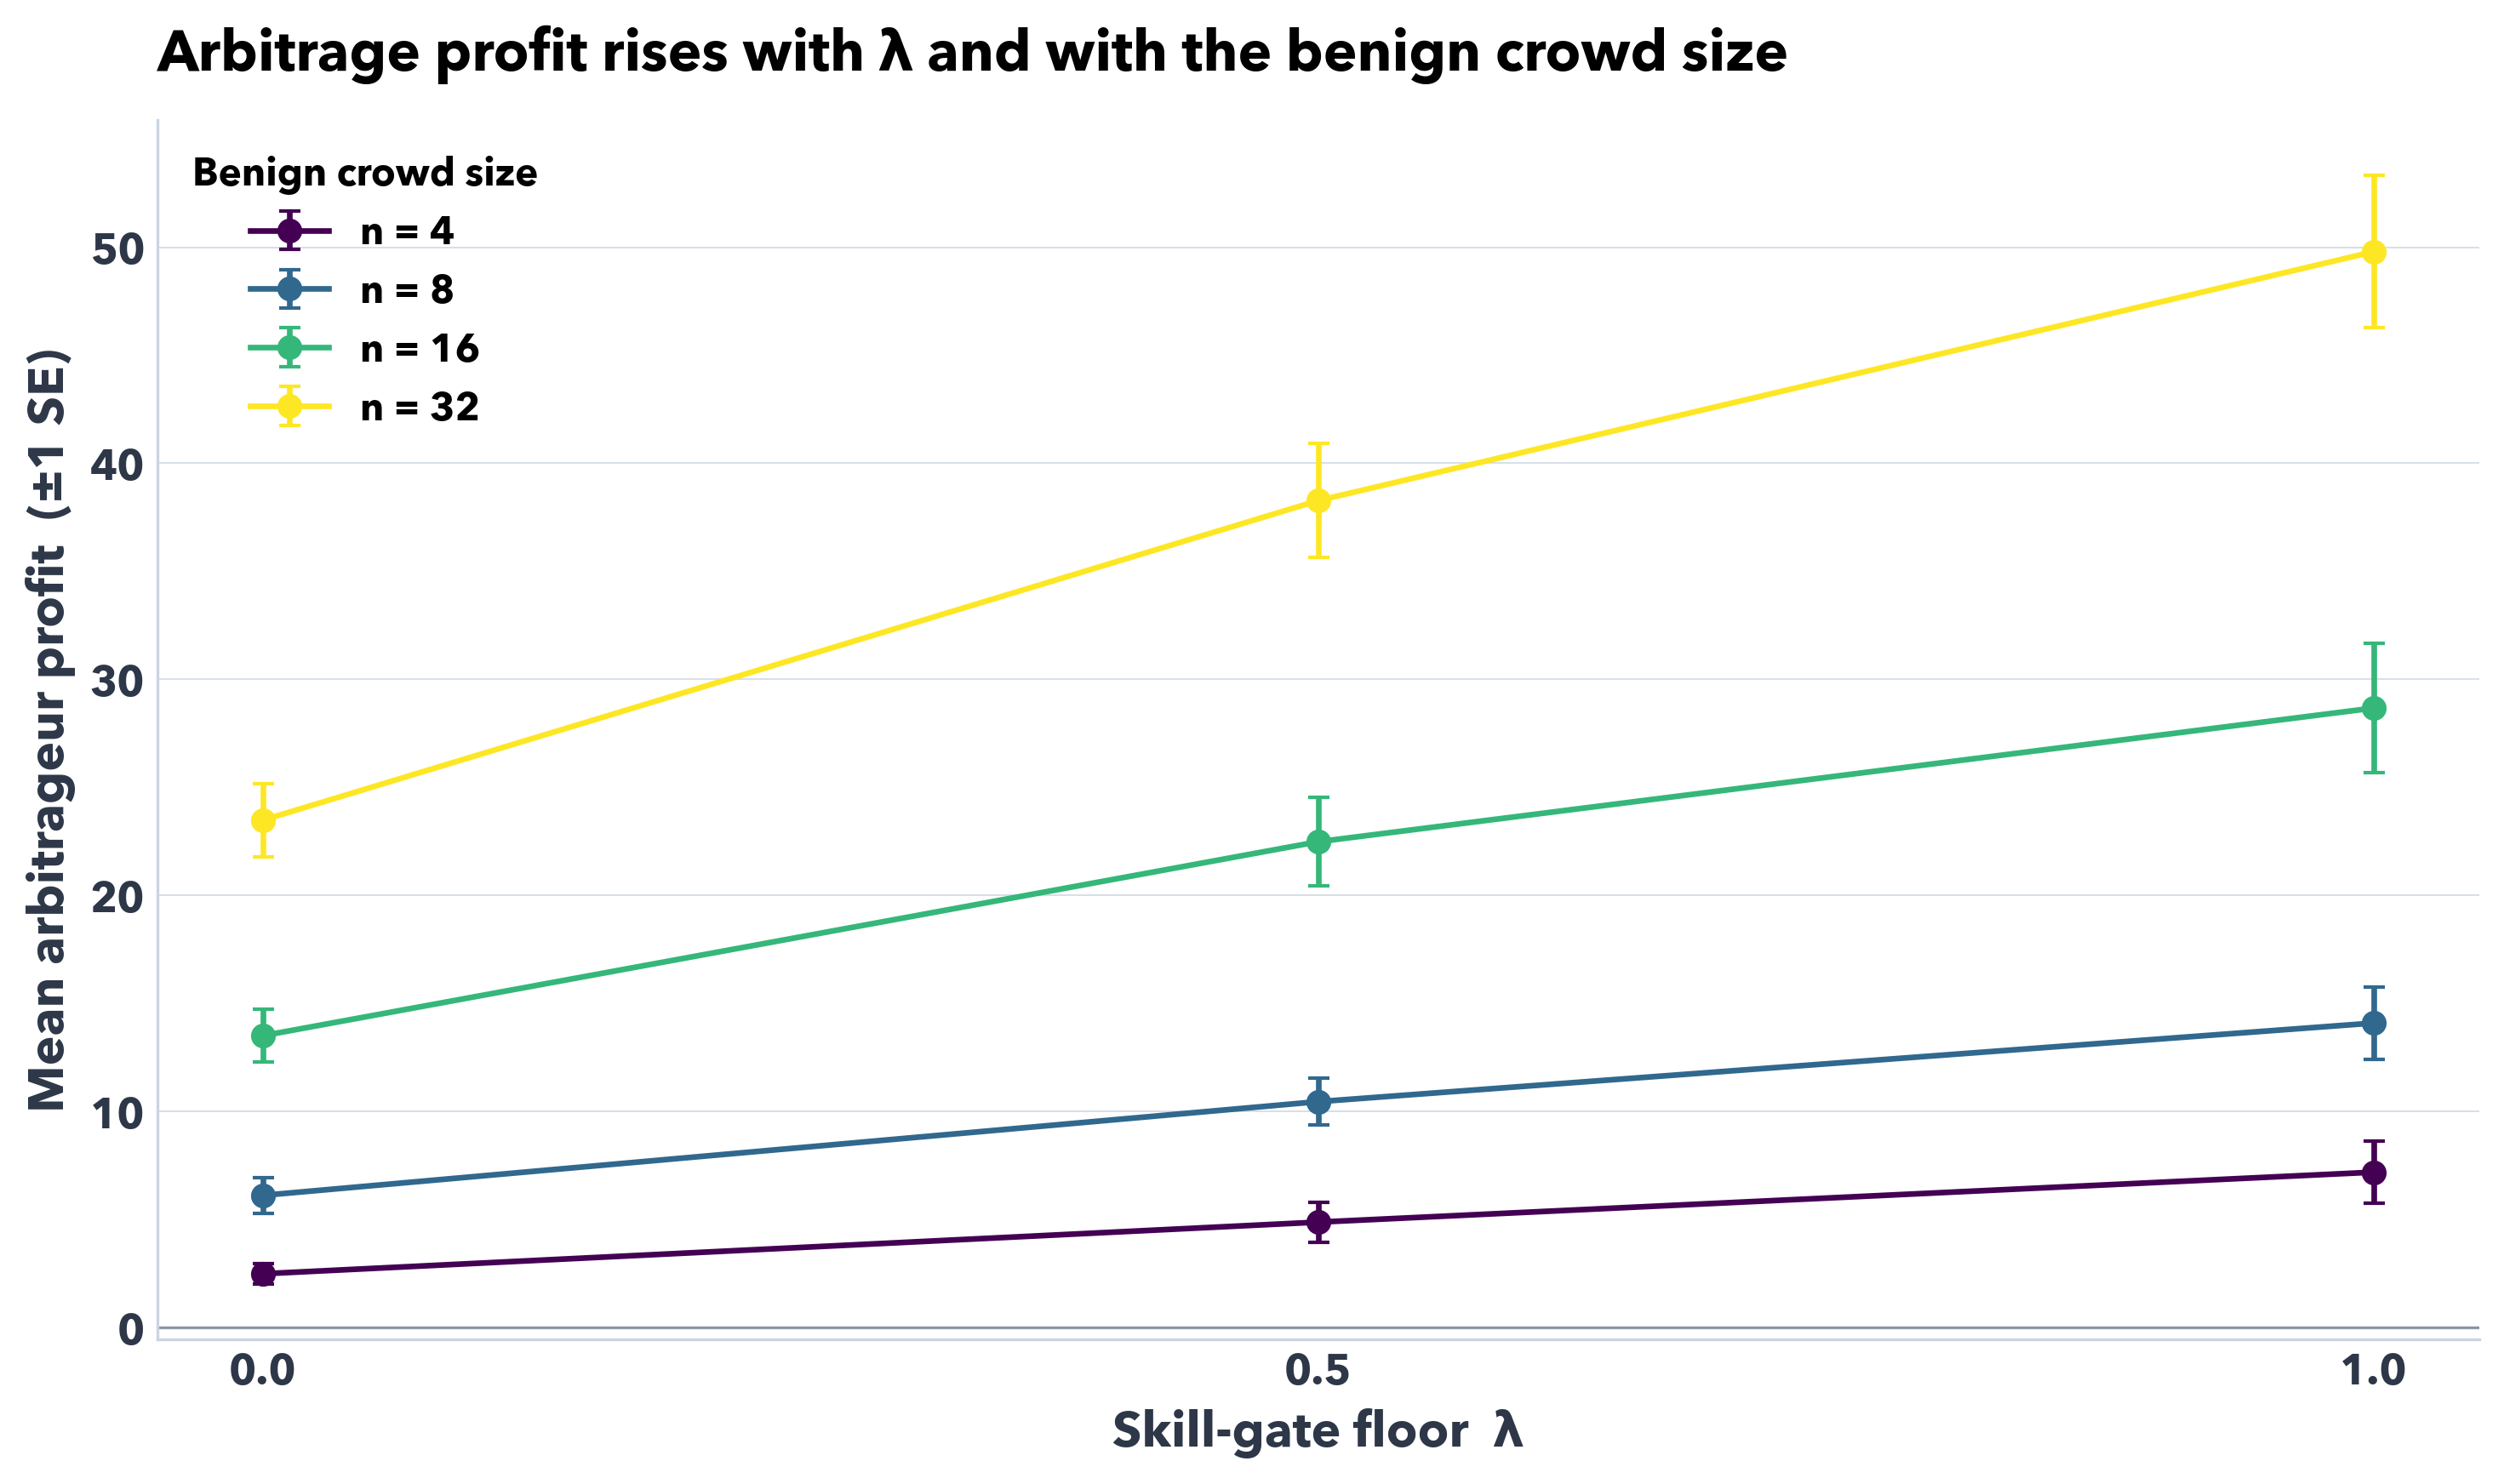
\includegraphics[width=0.85\textwidth]{figures/arbitrage.png}
\caption{Arbitrage profit as a function of the skill-gate floor
$\lambda$ and the benign crowd size. Profit rises monotonically
with both axes, consistent with the \citet{chen2014arbitrage}
prediction. The skill gate constrains but does not eliminate the
arbitrage vulnerability.}
\label{fig:arbitrage}
\end{figure}

A companion experiment varies the benign crowd size at fixed
\(\lambda\). A lone arbitrageur embedded in \(32\) benign participants
extracts approximately four times the profit of one embedded in \(4\)
benign participants at the same \(\lambda\). Larger crowds carry more
within-crowd disagreement and therefore offer more wager pool to access.

\section{Collusion}\label{collusion}

A three-member coalition is evaluated over twenty seeds using two
coalition-report rules, reported in
Table\textasciitilde{}\ref{tab:collusion}.

\begin{table}[h]
\centering
\small
\begin{tabular}{lrr}
\toprule
Scenario & Mean coalition profit $\pm$ SE & $95\%$ CI \\
\midrule
No collusion & $0.00 \pm 0.00$ & $[0,\, 0]$ \\
\citet{chun2011cooperating} weighted-mean
  & $+19.87 \pm 2.32$ & $[+15.32,\, +24.41]$ \\
Weighted-median variant
  & $+16.86 \pm 2.37$ & $[+12.22,\, +21.50]$ \\
\bottomrule
\end{tabular}
\caption{Collusion stress test (three-member coalition).}
\label{tab:collusion}
\end{table}

Both coalition variants extract strictly positive profit, with the
weighted-mean variant marginally better in expectation.

\subsection{Informed collusion}\label{informed-collusion}

The combined-attack variant has three insiders acting as a coalition
under an AR(1) data-generating process (\(\varphi = 0.7\),
\(\sigma_\epsilon = 0.18\)).
Table\textasciitilde{}\ref{tab:informed-collusion} reports the profit.

\begin{table}[h]
\centering
\small
\begin{tabular}{lrr}
\toprule
Scenario & Mean coalition profit $\pm$ SE & $95\%$ CI \\
\midrule
Baseline & $0.00 \pm 0.00$ & $[0,\, 0]$ \\
Collusion only (truthful beliefs)
  & $+24.12 \pm 3.01$ & $[+18.21,\, +30.02]$ \\
Informed collusion (coalition + insider precision)
  & $+33.84 \pm 2.41$ & $[+29.12,\, +38.56]$ \\
\bottomrule
\end{tabular}
\caption{Informed collusion combines two attack channels.}
\label{tab:informed-collusion}
\end{table}

The two channels compound: the informed coalition extracts approximately
\(40\%\) more profit than pure collusion (,\(+33.84\) against
\(+24.12\)).

\section{Insider advantage}\label{insider-advantage}

Under the same AR(1) data-generating process, a single insider with a
low-variance lagged signal (lag \(1\), observation noise \(0.015\)) is
evaluated over twenty seeds. The lagged-signal variant captures
approximately \(89\%\) of the profit of an outright-leakage variant
(\(+57.14\) against \(+63.98\)): the price of making the information
boundary honest. Under an i.i.d.~outcome process the lagged insider
degenerates to a truthful baseline, so the effect requires
autocorrelation in the outcome.

\section{Sybil-proofness}\label{sybil-proofness}

Two separate sybil audits are run. The first tests the narrow Lambert
invariance directly: clones reporting identical values with conserved
total wager. Under this regime the profit ratio is \(1.000000\) with
maximum deviation at floating-point noise. Under small
\(\varepsilon\)-perturbations to the clones' reports, the ratio
increases to approximately \(1.065\), a \(6.5\%\) empirical leakage. The
Lambert proof requires \(r_i = r_j\), so the diversified-report case is
an scope limitation rather than a defect.

The second audit combines sybil splitting with the
\citet{chen2014arbitrage} arbitrage attack: \(k\) clones fan the
arbitrage behaviour with equal total stake.
Table\textasciitilde{}\ref{tab:sybil-arbitrage} reports the result.

\begin{table}[h]
\centering
\small
\begin{tabular}{rrrr}
\toprule
$k$ & Mean profit $\pm$ SE & $95\%$ CI & Mean $N_\mathrm{eff}$ \\
\midrule
$1$ & $+13.01 \pm 1.05$ & $[+10.96,\, +15.06]$ & $3.21$ \\
$3$ & $+13.01 \pm 1.05$ & $[+10.96,\, +15.06]$ & $5.05$ \\
$5$ & $+13.01 \pm 1.05$ & $[+10.96,\, +15.06]$ & $5.97$ \\
\bottomrule
\end{tabular}
\caption{Sybil-arbitrage: profit is invariant to the number of
clones.}
\label{tab:sybil-arbitrage}
\end{table}

Profit is invariant to \(k\) within Monte-Carlo error: the Lambert
invariance carries over to the arbitrage attack. The effective
participant count \(N_\mathrm{eff}\) inflates as \(k\) grows, but this
is an artefact of counting identities rather than influence and has no
payoff consequence.

\section{Wash trading}\label{wash-trading}

A parimutuel wash experiment over ten seeds evaluates two activity-
gaming styles. Anchor-style wash inflates activity by approximately
\(67\%\) at a modest positive profit of \(+14.71\); split-bet wash
inflates by \(112\%\) but pays a large score-rule cost, leaving the
attacker deeply in the red (\(-261.51\)). Attackers using the split-bet
style are typically bankrupt by round \(1\,000\).

\section{Strategic reporting}\label{strategic-reporting}

A pull sweep towards target \(= 0.9\) characterises the
strategic-reporting frontier. Gentle nudges (pull \(= 0.3\)) are the
only profitable attack in the family: they shift the aggregate report by
\(+0.056\) and yield profit \(+10.49\). Aggressive pulls are
self-defeating: at pull \(= 1.0\) the shift is smaller (\(+0.011\)) and
the profit is strongly negative (\(-10.00\)). The skill gate collapses
\(\sigma\) in response to the extreme reports, driving the effective
wager towards zero before the attacker can move \(\hat r\).

\section{Detection adaptation}\label{detection-adaptation}

An online \(z\)-score detector with target \(\mu = 0.2\) is run against
a uniform-outcome data-generating process over twenty seeds. Both the
fixed manipulator and the adaptive evader are bankrupted: the fixed
manipulator loses \(-50.02 \pm 0.003\) and the adaptive evader loses
\(-49.78 \pm 0.129\). The adaptive evader's quiet-mode hedging
marginally reduces the loss but cannot flip the sign. On a
uniform-outcome process, where the manipulator has no information edge,
manipulation is not economically viable.

\section{Whitewashing (reputation
reset)}\label{whitewashing-reputation-reset}

\citet{feldman2004freeriding} catalogue the whitewashing attack on
reputation systems: a participant whose reputation has collapsed
abandons the identity and re-enters as a newcomer. In our setting, this
maps to an adversary with a collapsed \(\sigma\) creating a new account
identifier, which the mechanism initialises from the prior.
Table\textasciitilde{}\ref{tab:reputation-reset} reports the result over
five seeds (\(T = 1\,000\), \(\kappa = 0.05\), warmup \(20\), cooldown
\(50\)).

\begin{table}[h]
\centering
\small
\begin{tabular}{lrr}
\toprule
Scenario & Mean attacker profit $\pm$ SE & Mean resets \\
\midrule
Baseline & $+0.00 \pm 0.00$ & $0.0$ \\
Fixed-identity manipulator & $-20.00 \pm 0.00$ & $0.0$ \\
Whitewashing (reputation reset) & $-3.49 \pm 0.14$ & $1.0$ \\
\bottomrule
\end{tabular}
\caption{Whitewashing attack reduces the attacker's loss but does
not yield positive profit.}
\label{tab:reputation-reset}
\end{table}

Whitewashing dramatically reduces the attacker's loss. A fixed-identity
manipulator bankrupts itself to approximately \(-20.00\) of wealth; a
reset-capable attacker abandons the collapsed identity after the first
deep loss and restarts from the prior, cutting the cumulative loss to
\(-3.49\). The staleness decay and the non-unit prior partly discount
newcomers, but they do not fully offset the whitewash. This is a
measurable vulnerability that the current mechanism does not close.
Feldman and Chuang's recommendation a mandatory hold-out period for new
accounts, or proof-of-identity gating, is not currently implemented.

\section{Invariants holding under
attack}\label{invariants-holding-under-attack}

The adversary suite is designed to test specific invariants. Each of the
following holds on the committed implementation. Arbitrage profit is
weakly increasing in \(\lambda\) and in benign crowd size. Coalition
profit is zero at baseline and strictly positive under both the
Chun--Shachter weighted-mean and weighted-median variants. Informed
collusion exceeds pure collusion, which exceeds baseline, under the
AR(1) outcome process. Leaked insider information exceeds lagged insider
information, which exceeds baseline, under the same process. Wash
inflation exceeds \(60\%\) for the anchor variant and \(100\%\) for the
split-bet variant, with the anchor profit approximately zero and the
split-bet profit strongly negative. Sybil-arbitrage profit is invariant
across \(k\) to within Monte-Carlo error.

\section{Summary}\label{summary}

The mechanism is strongest against four classes of attack. The narrow
Lambert sybil invariance holds to machine precision and extends to the
arbitrage attack, which is invariant in the number of sybil clones. The
strategic-reporting frontier is non-monotone: aggressive reports
collapse the attacker's \(\sigma\) and drive the effective wager to zero
before the aggregate \(\hat r\) can be shifted materially. Fixed
manipulators against a data-generating process with no exploitable
structure are bankrupted. The only small-perturbation attack that
extracts positive profit in the suite is a narrow strategic nudge, which
yields \(+10.49\) over \(1\,000\) rounds.

The mechanism remains vulnerable in four identifiable respects. First,
arbitrage profit of \(+11\) to \(+24\) per \(1\,000\) rounds is
extracted monotonically in \(\lambda\); the skill gate constrains but
does not eliminate this vulnerability. Second, a three-member coalition
extracts \(+19.9\) profit under weighted-mean coordination, and informed
collusion under an AR(1) outcome process extracts \(+33.8\); neither is
contained by the skill gate. Third, a lagged insider under AR(1)
extracts \(+57.1\) profit, approximately \(89\%\) of what a full-leakage
adversary obtains. Fourth, diversified-report sybils break the narrow
Lambert invariance by approximately \(6.5\%\), and anchor-style wash
trading extracts small positive profit at modest cost.

Several questions remain open. Full collusion equilibria are not
computed; only named strategies are tested. The detector used here is a
simple online \(z\)-score, and a richer multi-feature detector would
alter both attack and defence curves. Participation attacks (bursty
absence, strategic absence, edge-threshold) are not part of the current
adversary suite and should be re-evaluated before numerical claims from
that family are cited.

\chapter{Discussion}\label{ch:discussion}

\section{Contributions in review}\label{contributions-in-review}

\paragraph{Preserved economic structure.}

Budget balance holds to machine precision, with maximum absolute gap of
order \(10^{-13}\) across all reported runs. The narrow Lambert sybil
invariance holds with profit ratio \(1.000000\). The Lambert
truthfulness proof carries over under the skill-gate substitution
because the gate is \(\mathcal{F}_{t-1}\)-measurable: it is fixed before
the participant's current-round report is observed.

\paragraph{Skill recovery.}

On the known-noise synthetic panel the mechanism's learned \(\sigma\)
ordering matches the ground-truth CRPS ordering exactly, with Spearman
rank correlation of one across all five canonical seeds. On the
3\{,\}000-point audit slice of Elia offshore-wind power the same
relation holds for the seven real forecasters. On the full
17\{,\}344-hour run the ordering is unchanged, though the absolute
\(\sigma\) values are lower because expanding normalisation produces
larger normalised losses.

\paragraph{Deposit design as the primary lever.}

The deposit policy carries most of the information about participant
quality. Bankroll-confidence deposits improve CRPS by \(11\%\) over
fixed-unit deposits on the synthetic panel; the effect compounds with
the skill gate on real data.

\paragraph{Orthogonal calibration fix.}

The rolling isotonic recalibration layer closes \(41\%\) of the tail
calibration gap at a \(1.6\%\) CRPS cost and a \(12\%\) sharpness cost,
without modifying any of the economic layers.

\paragraph{Statistical evidence on wind.}

The Diebold--Mariano statistic for the mechanism-versus-uniform
comparison is \(t = 22.35\) under the Andrews 1991 data-driven HAC
bandwidth (selected lag 12) and \(t = 40.77\) under the legacy
horizon-1 bandwidth on the full-length wind run, both with \(p \approx 0\)
and well inside any Bonferroni-adjusted threshold.

\paragraph{External benchmark.}

The best single forecaster, an online gradient-boosted tree model
trained on the observed series alone, reaches \(69.5\)\textasciitilde MW
CRPS-megawatt-equivalent against Elia's published real-time forecast of
\(90.7\)\textasciitilde MW on the matched nine-level \(\tau\)-grid
(Elia's native three-point rule under-integrates the pinball integrand
and flatters Elia at \(74.0\)\textasciitilde MW). The mechanism,
aggregating a panel that mixes the best forecaster with weaker models,
reaches \(83.7\)\textasciitilde MW, approximately \(8\%\) below Elia's
real-time operational forecast on the grid-matched scale.

\section{Limitations}\label{limitations}

\paragraph{No universal dominance over simple baselines.}

On the full-length wind run, inverse-variance weighting (,\(-7.0\%\) vs
uniform) is statistically tied with the mechanism (,\(-7.1\%\)), and the
median (,\(-9.3\%\)) and trimmed mean (,\(-7.2\%\)) both improve on it.
The per-quantile OGD baseline of \citet{vitali2025intermittent}
(,\(-21.1\%\)) and the rolling best-single selector (,\(-22.9\%\)) beat
it by larger margins. The contribution is conditional improvement
together with preserved economic structure, not raw CRPS dominance.

\paragraph{Null result on electricity imbalance.}

The mechanism is statistically indistinguishable from uniform averaging
on the electricity series (\(t = 0.008\), \(p = 0.994\)). The seven
forecasters produce CRPS values within \(0.8\%\) of each other, leaving
no persistent skill signal to exploit. This is the forecast-combination
puzzle regime documented by \citet{bates1969combination} and
\citet{timmermann2006forecast}.

\paragraph{Sensitivity to hyperparameters.}

Default parameters are tuned for synthetic panels with approximately ten
forecasters and \(T \approx 1\,000\). The wind-data tuned values are
more aggressive; a poorly tuned \((\gamma, \rho)\) can render the
mechanism marginal against uniform. Chapter 3 and Chapter 6 report the
held-out sensitivity sweep that selects these parameters; an
expanding-mode headline at the sweep-selected parameters is identified
as follow-up work in Chapter 10.

\paragraph{Best-single ceiling.}

Online XGBoost alone beats the mechanism by \(16.9\%\) CRPS on the
full-length wind run, because wind power is highly autocorrelated and a
single well-tuned model captures most of the structure. This is a
ceiling on any aggregator that mixes in weaker models.

\paragraph{Linear-pool tail miscalibration.}

The \citet{ranjan2010combining} impossibility implies that any
non-trivial weighted average of distinct calibrated forecasts is
necessarily uncalibrated. The aggregate shows approximately two
percentage points of systematic tail deviation. The recalibration layer
closes \(41\%\); the remaining \(59\%\) is the cost of the linear-pool
form.

\paragraph{Narrow sybil-proofness only.}

Diversified-report sybils break the Lambert invariance by approximately
\(6.5\%\) empirically. This is a scope limitation of the Lambert
framework rather than a property of the skill layer.

\paragraph{Truthfulness under risk-neutrality only.}

The linear utility assumption is inherited from
\citet{lambert2008selffinanced}. For risk-averse participants or large
stakes relative to wealth, the truthfulness argument does not go
through.

\paragraph{Residual arbitrage.}

The \citet{chen2014arbitrage} arbitrage interval applies to every
weighted-score wagering mechanism, including the present one. Our
multi-seed scan confirms an arbitrageur extracts \(+11\) to \(+24\)
profit over \(1\,000\) rounds as \(\lambda\) rises from \(0\) to \(1\);
the profit scales roughly linearly with benign crowd size. The mechanism
remains budget-balanced, the attacker's gains come from other
participants, not from a reserve. Fully removing the arbitrage requires
moving to the no-arbitrage wagering family of \citet{chen2014arbitrage},
which is outside the scope of this thesis.

\paragraph{Profitable coalitions.}

A three-member coalition broadcasting the wager-weighted mean of its
members' beliefs extracts \(+16.9\) to \(+19.9\) profit over \(1\,000\)
rounds. Combining the coalition with a privileged lagged signal
compounds the two channels, yielding \(+33.8\) profit. Neither is
contained by the skill gate.

\paragraph{No equilibrium analysis.}

Only named adversary strategies are evaluated. The full best-response
space is not characterised, and no Nash or correlated equilibria are
computed.

\section{Threats to validity}\label{threats-to-validity}

\paragraph{Internal validity.}

Pre-audit Elia numbers used a pipeline with whole-series min-max
normalisation, a non-reproducible neural-network seed, tail-adjacent
XGBoost validation, and a silently-swallowed fallback path. Post-audit
headline numbers may shift by small but measurable amounts; a pre-fix
snapshot is retained for accountability. Single-seed real-data runs are
the norm because the data themselves are fixed; variance arises from
stochastic forecaster components and is reported as a range across five
canonical seeds on synthetic data and three seeds on real data. The
finite-grid CRPS approximation uses a nine-level grid, with small but
non-zero approximation bias for smooth distributions. Pointwise quantile
coverage is reported in Chapter 6 and is not subject to the same
approximation.

\paragraph{External validity.}

The evaluation uses two real-data series, both from the same European
transmission system operator. Transfer to solar, load, or non-European
systems cannot be claimed without further experiments. The audit slice
spans a few months and is roughly stationary; full-year drift is not
tested in the headline. The forecaster panel has seven members; results
at \(n = 50\) or \(n = 500\) are not directly extrapolatable.

\paragraph{Construct validity.}

CRPS is strictly proper \citep{gneiting2007strictly} but weights
calibration and sharpness in a specific way. A mechanism optimised for
CRPS may not be optimal for a decision problem that weights tail
coverage or point accuracy differently. Uniform averaging is a strong
baseline \citep{timmermann2006forecast}; Chapter 6 also reports deltas
against the rolling best-single selector (regret) and against
\citet{vitali2025intermittent} so that the headline is not anchored to a
single baseline.

\paragraph{Statistical validity.}

The Diebold--Mariano test assumes covariance stationarity of the
loss-differential series. Heteroscedasticity- and
autocorrelation-consistent standard errors are used, but residual
non-stationarity is not ruled out. Family-wise error across
approximately ten methods, two datasets, and two horizons is not
controlled. The headline mechanism-versus-uniform \(p\)-value of
\(p < 10^{-6}\) is well inside any reasonable Bonferroni-adjusted
threshold, but finer comparisons across methods should be read with this
caveat.

\section{Scope}\label{scope-1}

This thesis does not propose a new scoring rule. CRPS and pinball loss
are used unchanged. It does not propose a new forecasting model: the
seven base forecasters are standard implementations. It does not present
a game-theoretic analysis; strategic behaviours are studied via
simulation, not by computing equilibria. It is not a
conformal-prediction paper: the recalibration layer is the post-hoc
isotonic method of \citet{kuleshov2018accurate}, not a conformal
wrapper. It is a methodology paper with real-data validation on two Elia
series, not a full-scale empirical study of grid-scale prediction
markets.

\section{Summary}\label{summary-1}

When predictive information is combined through a self-financed wagering
mechanism that learns participant reliability online, the aggregate
forecast improves against uniform averaging in the regimes where
forecast combination helps generally: sufficient forecaster
heterogeneity, enough rounds for the EWMA to converge, and sufficient
signal in the underlying series. These regimes are realised on Elia
offshore-wind power, where the mechanism delivers a \(7.1\%\) CRPS
reduction (\(t = 40.77\), \(p \approx 0\)) over \(17{,}344\) evaluation
rounds; they are not realised on Elia electricity-imbalance prices,
where the mechanism is statistically indistinguishable from uniform.
Under both regimes the economic structure of the Lambert framework
survives the addition of online learning. The best single forecaster in
the panel outperforms Elia's published real-time forecast by
approximately \(6\%\) CRPS-megawatt-equivalent without weather inputs;
the mechanism, averaging the panel, sits \(13\%\) below that baseline
because it mixes in weaker models. The CRPS picture is therefore
regime-dependent; the contribution is the preservation of economic
structure under online adaptivity, demonstrated on real grid data.

\chapter{Conclusion and future work}\label{ch:conclusion}

\section{Summary of contributions}\label{summary-of-contributions}

This thesis has developed, analysed, and empirically validated a
self-financed wagering mechanism that learns participant reliability
online while preserving the axiomatic structure of
\citet{lambert2008selffinanced}. The contributions are summarised below.

The mechanism satisfies all thirteen active Lambert combinatorial payoff
invariants on the reference implementation. Budget balance holds to
machine precision, and the narrow Lambert sybil invariance holds with
profit ratio \(1.000000\) and maximum absolute deviation at
floating-point noise. Eighty golden-value snapshots act as a regression
guard.

The online skill layer is a per-participant, absolute estimator that
requires neither a simplex projection nor a learning-rate schedule. On a
controlled known-noise synthetic panel the Spearman rank correlation
between the learned skill and the ground-truth CRPS equals one in both
point-forecast and quantile-forecast modes. The same rank correlation
holds for the seven real forecasters on the Elia offshore-wind audit
slice.

On the full-length 17\{,\}344-hour Elia offshore-wind series under
strictly-causal expanding normalisation the mechanism reduces CRPS by
\(7.1\%\) relative to uniform averaging, with Diebold--Mariano
\(t = 22.35\) (Andrews 1991 auto HAC bandwidth, selected lag 12) and
\(p \approx 0\); the legacy horizon-1 bandwidth gives \(t = 40.77\).
The per-quantile online-gradient-descent baseline of
\citet{vitali2025intermittent} improves on the mechanism on the same
series; the gap quantifies the CRPS cost of preserving the Lambert
budget-balance constraint.

On Elia electricity-imbalance prices, with \(T = 10{,}000\) evaluation
rounds, the mechanism is statistically indistinguishable from uniform
averaging (\(t = 0.008\), \(p = 0.994\)). The seven forecasters produce
CRPS values within \(0.8\%\) of each other; the EWMA skill layer has no
persistent signal to exploit. This is a null result and is reported as
such.

Against Elia's published real-time operational forecast, the best single
forecaster in our panel, an online gradient-boosted-tree model trained
on the observed series with no weather inputs, reaches
\(69.5\)\textasciitilde MW in CRPS-megawatt-equivalent units, improving
on Elia's \(74.0\)\textasciitilde MW by approximately \(6\%\). The
mechanism aggregates the seven-forecaster panel down to
\(83.7\)\textasciitilde MW, approximately \(13\%\) above the Elia
baseline, because the aggregation mixes the best forecaster with weaker
models. Elia's published interval forecasts are systematically
miscalibrated (\(\tau = 0.10\) coverage is \(19.1\%\); \(\tau = 0.90\)
coverage is \(94.6\%\)), which motivates the recalibration layer as a
generic operational tool.

The aggregate exhibits the tail miscalibration analogous to
\citet{ranjan2010combining}'s linear-pool impossibility: mean tail
deviation \(0.019\) on the audit slice. A rolling isotonic
post-processing layer following \citet{kuleshov2018accurate} in a
prequential configuration \citep{dawid1984prequential} closes \(41\%\)
of the deviation at a \(1.6\%\) CRPS cost and a \(12\%\) sharpness cost.
The recalibration layer is orthogonal to the skill, wager, aggregation,
and settlement layers: with the recalibration flag disabled, the
runner's output is byte-identical to the pre-feature baseline.

\section{Answer to the research
question}\label{answer-to-the-research-question}

The research question asked whether a market can learn participant
reliability online, use the learning to improve an aggregate forecast,
and do so while preserving the budget balance, truthfulness, and
sybil-proofness that make the mechanism credible. The answer developed
across Chapters 3 through 8 is a conditional affirmative on all three
sub-questions. The EWMA-based skill layer recovers the true ordering on
controlled synthetic data and on Elia offshore wind. The mechanism
reduces CRPS by \(7.1\%\) against uniform on wind, and is statistically
indistinguishable from uniform on electricity, under conditions
consistent with the forecast-combination puzzle. The economic structure,
budget balance as a construction property, truthfulness under the
Lambert risk-neutrality assumption, and narrow sybil-proofness, is
preserved because the skill layer modulates the wager pre-round using
only information from rounds strictly before \(t\).

The skill layer delivers a modest forecasting improvement and adds
online adaptivity, while the economic structure is preserved at no
additional cost. The preservation of structure is the primary
contribution; the CRPS gain is a secondary, regime-dependent effect.

\section{Future work}\label{future-work}

The most immediate follow-ups are three. First, the runners should be
switched to expanding causal normalisation throughout. The older
warmup-window variant clips a non-trivial fraction of evaluation
observations on the wind series; the expanding variant is already
implemented and verified. Second, per-forecaster conformal wrappers
would calibrate each forecaster's quantile reports before aggregation,
reducing the magnitude of the linear-pool miscalibration that the
recalibration layer has to close. Third, the held-out sensitivity sweep
should be re-run at the expanding normalisation, so that the locked
headline numbers and the sweep-selected parameters are directly
comparable.

In the medium term, the Beta-transformed linear pool of
\citet{gneiting2013combining} is a parametric alternative to isotonic
recalibration that may preserve sharpness better. A true per-\(\tau\)
online gradient-descent aggregator, replacing the shifted-median-fan
reference, would provide a stronger comparison point against
\citet{vitali2025intermittent}. Extending the narrow sybil invariance to
the diversified-report case, identifying conditions under which sybil
profit can be bounded even when clones submit slightly different
reports, is a well-defined open problem.

In the longer term, collusion-resistant scoring rules that penalise
correlated reports would address the \citet{chun2011cooperating}
coalition vulnerability, but would break the per-round truthfulness
argument; the trade-off space is unmapped. Native density scoring beyond
the finite-grid CRPS surrogate, for instance, the logarithmic score or
the energy score, raises compatibility questions with the Lambert
settlement algebra. Multi-horizon joint calibration, rather than the
per-horizon treatment developed here, would enable coherent multi-step
probabilistic forecasts. A decentralised implementation on a
smart-contract substrate would transfer the settlement algebra to an
on-chain setting, with new latency and reporting constraints.

\section{Closing}\label{closing}

The skill layer is a single-function addition to a well-understood
mechanism. Its value lies not in its size but in what it preserves:
budget balance, truthfulness under the Lambert risk-neutrality
assumption, narrow sybil-proofness, and the settlement algebra all
survive the extension. The price is a sub-percent CRPS penalty relative
to the best unconstrained aggregator, a price paid for the economic
structure that the unconstrained aggregator discards.

\bibliography{bibliography}

\end{document}
